\documentclass[12pt]{report}


\usepackage[utf8]{inputenc}
\usepackage{anyfontsize}
\usepackage[italian]{babel}
\usepackage[a4paper, top=3.0cm, bottom=3.5cm, left=3.5cm, right=3.5cm, footskip=2cm]{geometry}
\usepackage{amsmath}
\usepackage{graphicx}
% \usepackage[colorlinks=true, allcolors=blue]{hyperref}
\usepackage[colorlinks=false]{hyperref}
\usepackage{xurl}
\usepackage{listings}
\usepackage{textcomp}
\usepackage{scrextend}
\usepackage{xspace}
\usepackage{hyperref}
\usepackage[nameinlink]{cleveref}
\usepackage{pifont}
\usepackage{caption}
\usepackage{noindentafter}
\usepackage[explicit,noindentafter]{titlesec}
\usepackage{mdframed}
\usepackage{xcolor}
\usepackage{lmodern}
\usepackage{float}
\usepackage[backend=bibtex, style=numeric]{biblatex}
\usepackage{enumitem}
\usepackage{cleveref}


\addbibresource{refs.bib}


\crefname{figure}{Figura}{Figure}
\crefname{section}{Sezione}{Sezioni}
\crefname{chapter}{Capitolo}{Capitoli}
\crefname{appendix}{Appendice}{Appendici}
\crefrangeformat{section}{da~#3#1#4 a~#5#2#6}  %usare questo per il plurale


\mdfsetup{
    innerleftmargin=25pt,
    innerrightmargin=25pt,
    innertopmargin=20pt,
    innerbottommargin=20pt
}


\lstset{
    literate=%
    {à}{{\`a}}1
    {è}{{\`e}}1
    {ì}{{\`i}}1
    {ò}{{\`o}}1
    {ù}{{\`u}}1
    {á}{{\'a}}1
    {é}{{\'e}}1
    {í}{{\'i}}1
    {ó}{{\'o}}1
    {ú}{{\'u}}1
    {À}{{\`A}}1
    {È}{{\`E}}1
    {Ì}{{\`I}}1
    {Ò}{{\`O}}1
    {Ù}{{\`U}}1
    {Á}{{\'A}}1
    {É}{{\'E}}1
    {Í}{{\'I}}1
    {Ó}{{\'O}}1
    {Ú}{{\'U}}1
}


\titleformat{\chapter}[frame]{\Huge\scshape}{\filcenter\thechapter}{30pt}{\filcenter #1}{}
\titlespacing{\chapter}{0pt}{80pt}{40pt}
\NoIndentAfterEnv{chapter}
\captionsetup{font=footnotesize}


\newcommand{\torevise}[1]{\textcolor{red}{#1}}
\newcommand{\edit}[1]{\textcolor{NavyBlue}{#1}}
\newcommand{\stable}[1]{\textcolor{black}{#1}}


\newcommand{\myref}[1]{\textsuperscript{\hyperref[#1]{\ding{70}}}}

\newcommand{\toody}{\textsl{TooDY}\xspace}
\newcommand{\python}{\textsl{Python}\xspace}
\newcommand{\jinja}{\textsl{Jinja}\xspace}
\newcommand{\javascript}{\textsl{JavaScript}\xspace}
\newcommand{\flask}{\textsl{Flask}\xspace}
\newcommand{\django}{\textsl{Django}\xspace}
\newcommand{\spacy}{\textsl{spaCy}\xspace}
\newcommand{\nltk}{\textsl{NLTK}\xspace}
\newcommand{\sple}{\textsl{SPLE}\xspace}
\newcommand{\spl}{\textsl{SPL}\xspace}
\newcommand{\srs}{\textsl{SRS}\xspace}
\newcommand{\fast}{\textsl{FAST}\xspace}
\newcommand{\rseb}{\textsl{RSEB}\xspace}
\newcommand{\foda}{\textsl{FODA}\xspace}
\newcommand{\uml}{\textsl{UML}\xspace}
\newcommand{\nlp}{\textsl{NLP}\xspace}
\newcommand{\html}{\textsl{HTML}\xspace}
\newcommand{\json}{\textsl{JSON}\xspace}
\newcommand{\ace}{\textsl{ACE}\xspace}

\newcommand{\URL}{\textsf{URL}\xspace}
\newcommand{\api}{\textsf{API}\xspace}
\newcommand{\http}{\textsf{HTTP}\xspace}
\newcommand{\post}{\textsf{POST}\xspace}


\hyphenation{
    TooDY
    Python
    Jinja
    JavaScript
    Flask
    Django
    spaCy
    NLTK
    SPLE
    SPL
    SRS
    FAST
    RSEB
    FODA
    UML
    NLP
    HTML
    JSON
    ACE
    URL
    API
    HTTP
    POST
}


\definecolor{codegray}{rgb}{0.5,0.5,0.5}      % grigio
\definecolor{codeorange}{rgb}{0.6, 0.2, 0.0}  % arancione
\definecolor{codegreen}{rgb}{0, 0.4, 0}       % verde


\lstset{
    commentstyle=\color{codegray},    % colore commenti: grigio
    keywordstyle=\color{codeorange},  % colore parole chiave: arancione
    stringstyle=\color{codegreen},    % colore stringhe: verde
    basicstyle=\ttfamily\small,       % Imposta il font monospazio di dimensione piccola
    showspaces=false,                 % Non mostra gli spazi
    showtabs=false,                   % Non mostra i tab
    showstringspaces=false,           % Non mostra gli spazi nelle stringhe
    frame=none,                       % Aggiunge una cornice attorno al codice
    tabsize=4,                        % Imposta la dimensione del tab a 2 spazi
    keepspaces=true,                  % Mantiene gli spazi nel testo
    columns=flexible,                 % Colonne flessibili
    numbers=none,                     % Mostra i numeri di riga a sinistra
    numbersep=5pt,                    % Distanza tra i numeri di riga e il codice
}


\lstdefinelanguage{JavaScript}{
    keywords={
        break,
        case,
        catch,
        continue,
        debugger,
        default,
        delete,
        do,
        else,
        false,
        finally,
        for,
        function,
        if,
        in,
        instanceof,
        new,
        null,
        return,
        switch,
        this,
        throw,
        true,
        try,
        typeof,
        var,
        void,
        while,
        with
    },
    morecomment=[l]{//},
    morecomment=[s]{/*}{*/},
    morestring=[b]',
    morestring=[b]",
    ndkeywords={
        class,
        export,
        boolean,
        throw,
        implements,
        import,
        this
    },
    keywordstyle=\color{codeorange}\bfseries,
    ndkeywordstyle=\color{black}\bfseries,
    identifierstyle=\color{black},
    commentstyle=\color{codegray}\ttfamily,
    stringstyle=\color{codegreen}\ttfamily,
    sensitive=true
}


\begin{document}
\fontsize{13}{18}\selectfont


% PAGINA BIANCA
% \clearpage\thispagestyle{empty}
% \null\newpage


% FRONTESPIZIO
\begin{titlepage}
\begin{figure}
\centering
\includegraphics[scale=0.5]{cherubino.png}
\vspace{0.5cm}
\end{figure}
\begin{center}
{\large{UNIVERSITÀ DEGLI STUDI DI PISA}}\\
\vspace{0.5cm}
{\LARGE{Corso di Laurea in Informatica \textsl{L-31}}}\\
\vspace{2cm}
{\Large{TESI DI LAUREA}}\\
\vspace{2cm}
{\huge{\toody\\{\normalsize Tool for Detecting variabilitY}}}
\end{center}
\vspace{2cm}
\begin{minipage}[t]{0.49\textwidth}\centering
{\large{\scshape{Relatore}\\\bf{Prof.ssa Laura Semini}}}
\end{minipage}
\hfill
\begin{minipage}[t]{0.49\textwidth}\centering
{\large{\scshape{Candidato}\\\bf{Matteo Giorgi}}}
\vspace{4cm}
\end{minipage}
\centering{\large ANNO ACCADEMICO 2022/2023}
\end{titlepage}


% INIZIO NUMERAZIONE ROMANA
\pagenumbering{roman}


% PAGINA BIANCA
\clearpage\thispagestyle{empty}
\null\newpage


% INDICE
\tableofcontents


% PAGINA BIANCA
\clearpage\thispagestyle{empty}
\null\newpage

\clearpage\thispagestyle{empty}
\null\newpage


% SALVO NUMERO PAGINA
\newcounter{tempCntr}
\setcounter{tempCntr}{\value{page}}


% \color{blue}
% SOMMARIO
\begin{abstract}
\thispagestyle{plain}
\setcounter{page}{\value{tempCntr}}
Il lavoro si colloca in una linea di ricerca per la specifica di linee di prodotto software (\spl) a partire da documenti di requisiti in linguaggio naturale.

Le ambiguità in un documento dei requisiti normalmente causano incoerenze tra l'aspettativa del cliente e il prodotto sviluppato, e spesso portano a rielaborazioni indesiderate degli artefatti. Tuttavia, un termine ambiguo può anche essere usato come mezzo per rimandare una decisione. Sviluppando questa idea, è stato precedentemente mostrato che il rilevamento dell'ambiguità può anche essere usato come un modo per catturare aspetti nascosti di variabilità nei requisiti, usando nella ricerca indicatori specifici per la variabilità che sono una variazione rispetto agli indicatori di ambiguità noti.

In questo lavoro di tesi, partendo da un prototipo iniziale, è stato realizzato uno strumento di elaborazione del linguaggio naturale  per individuare, in un documento dei requisiti, indicatori di variabilità. Il tool realizza funzionalità di analisi lessicale e sintattica ed è  implementato usando la libreria \spacy.
\end{abstract}


% RIPRISTINO NUMERAZIONE ARABA
\pagenumbering{arabic}


% PAGINA BIANCA
\clearpage\thispagestyle{empty}
\null\newpage




% CAPITOLO 1
\chapter{Introduzione}
L’abilità di sviluppare software di qualità ha inizio con una definizione precisa ed esaustiva dei requisiti richiesti: il documento dei requisiti, in tal senso, rappresenta l'elemento base sul quale si fonda l’intero ciclo di vita del progetto software. La redazione di tale documento tuttavia, non è compito semplice e ciò è principalmente dovuto alla natura ambigua e intrinsecamente imprecisa del linguaggio naturale comunemente utilizzato per esprimerlo. In un progetto software la formalizzazione dei requisiti è dunque pratica essenziale e, se non opportunamente curata, veicolo di ambiguità che spesso portano a interpretazioni errate, incoerenze ed eventuali fallimenti nel soddisfare le aspettative del cliente.

La presente tesi si colloca in questo scenario e si basa su un precedente lavoro \cite{livi}, concluso con lo sviluppo di un piccolo script eseguibile da riga di comando. Sebbene tale script rappresentasse un passo iniziale promettente, era limitato in termini di interfaccia utente e flessibilità di utilizzo. Per questo motivo è stato esteso il progetto iniziale, trasformandolo in un'applicazione più robusta e versatile.

Il progetto implementa \toody (tool for detecting variability): una web-app focalizzata sull’identificazione della \textsf{Variabilità} nei documenti dei requisiti redatti in linguaggio naturale. L’obiettivo è quello di creare uno strumento facile e veloce da usare; un supporto concreto nell’analisi dei requisiti, utile ad individuare indicatori di variabilità. Questi indicatori corrispondono a punti di variabilità nella specifica di una linea di prodotti.


\section{Strumenti utilizzati}
Nell’ambito di questo progetto, sono stati utilizzati diversi strumenti che hanno facilitato lo sviluppo e la realizzazione del tool; tra questi, meritano una menzione particolare \flask e \spacy. \flask è un micro-framework per interfacce web, estremamente flessibile e leggero, che ha permesso di sviluppare un server dedicato all’elaborazione delle richieste relative all’analisi dei documenti dei requisiti e alla gestione di un database contenente lo storico di ciascun utente registrato al servizio web. L'utente può quindi modificare e analizzare i documenti caricati, verificandone la correttezza formale e controllandone i vari casi di ambiguità e variabilità. \spacy, invece, è una libreria open source di elaborazione del linguaggio naturale, che ha fornito le funzionalità di analisi lessicale e sintattica necessarie per l’individuazione degli indicatori di variabilità nei documenti analizzati. La scelta di tali strumenti è stata dettata dalla necessità di avere un sistema flessibile in grado di gestire analisi linguistiche complesse.

Unitamente a ciò, l'interfaccia intuitiva della web-app facilita l'interazione con il sistema, permettendo agli utenti di gestire i documenti direttamente sulla piattaforma ed eseguire l'analisi in modo semplice e diretto. La possibilità di visualizzare in tempo reale i risultati dell'analisi è certamente uno strumento utile per le fasi di verifica e validazione, promuovendo così un approccio più accurato e riflessivo nella definizione dei requisiti del software.


\section{Motivazioni}
L’idea alla base del progetto è quella di trasformare un termine ambiguo da ostacolo a risorsa, utilizzarlo come mezzo per rimandare alcune decisioni e, al contempo, identificare aspetti nascosti di variabilità nei requisiti.

Le richieste iniziali del progetto delineavano la necessità di una piattaforma facilmente accessibile attraverso diversi sistemi operativi e questo requisito ha orientato la scelta verso lo sviluppo di una web-app, permettendo così un accesso ubiquo e una fruibilità trasversale, indipendentemente dal sistema utilizzato. L'interfaccia così realizzata, non solo facilita l'interazione con il sistema di analisi, ma integra la gestione dei documenti, fornendo all'utente uno strumento completo per l'elaborazione dei testi.


\section{Struttura e contenuto}
La presente dissertazione è organizzata seguendo una logica chiara e progressiva, mirata a fornire una comprensione completa del lavoro svolto e degli obiettivi raggiunti con lo sviluppo di \toody.

% {\centering \rule{0.5\linewidth}{0.1pt} \par\vspace{0.25cm}}

\begin{mdframed}
\small
Il capitolo \textsf{\spl Engineering}\myref{ch:sple} approfondisce i vari paradigmi legati alle linee di prodotto software, esplorando metodologie come \textit{FAST}, \textit{RSEB} e \textit{FODA}. In particolare, si discutono le tecniche di analisi del dominio e la rappresentazione attraverso \textit{Features Diagrams}. Viene anche affrontata la tematica dell’ambiguità linguistica e come essa possa introdurre variabilità nei requisiti.

\vspace{0.25cm}

Nella sezione \textsf{\nlp \& \spacy}\myref{ch:nlp}, si esplorano le fondamenta dell'elaborazione del linguaggio naturale. Vengono presentate le principali tecniche e illustrato come queste siano state applicate per la realizzazione pratica del tool con l'ausilio della libreria \spacy.

\vspace{0.25cm}

% Concluso \torevise{Conclusa} l'introduzione teorica, nella sezione \textsf{\toody analyzer}\myref{ch:parser} vengono presentati i dettagli implementativi del tool di analisi che fanno uso proprio dei concetti esposti nei capitoli precedenti.
Conclusa l'introduzione teorica, nella sezione \textsf{\toody analyzer}\myref{ch:parser} vengono presentati i dettagli implementativi del tool di analisi che fanno uso proprio dei concetti esposti nei capitoli precedenti.

\vspace{0.25cm}

Il cuore della tesi è rappresentato da \textsf{\toody web-app}\myref{ch:architettura}. In questo capitolo si fornisce un'analisi tecnica dettagliata del progetto: sono presentate l’interfaccia utente e l'architettura del server \flask.

\vspace{0.25cm}

In ultimo, nella sezione \textsf{Conclusioni}\myref{ch:conclusioni} si riflette sulle competenze acquisite, sulle potenzialità di \toody e sugli sviluppi futuri, offrendo una visione d'insieme in merito alle implicazioni e alle prospettive del progetto.
\end{mdframed}

% {\centering \rule{0.5\linewidth}{0.1pt} \par\vspace{0.25cm}}

\noindent Attraverso l’implementazione di \toody, questo elaborato mira a fornire uno strumento utile ed efficace per l’identificazione della variabilità, con l’obiettivo di migliorare la qualità del processo di analisi dei requisiti e del software prodotto.

{\centering \rule{0.5\linewidth}{0.1pt} \par\vspace{0.25cm}}

\noindent Il codice sorgente dell'applicazione \toody è disponibile pubblicamente su GitHub all'indirizzo \url{https://github.com/matteogiorgi/toody}.


% PAGINA BIANCA
\clearpage\thispagestyle{empty}
\null\newpage




% CAPITOLO 2
\chapter{\spl Engineering}
\label{ch:sple}
Nell'ambito dello sviluppo software, la definizione e la comprensione dei requisiti sono fondamentali per garantire che il prodotto finale soddisfi le esigenze e le aspettative degli stakeholder. I requisiti sono specifiche formali di necessità o caratteristiche che un componente software deve possedere e sono essenziali per lo sviluppo del sistema: essi orientano il design, l'implementazione e la verifica del prodotto finale.

Nella fase iniziale dello sviluppo software viene redatto il documento dei requisiti che fornisce una descrizione dei \textit{requisiti funzionali} e dei \textit{requisiti non funzionali}\footnote{I \textit{requisiti funzionali} descrivono specifiche funzioni, comportamenti o servizi che un sistema software deve fornire. Definiscono \textit{cosa} il software dovrebbe fare, specificando le azioni che il sistema deve compiere in determinate condizioni.\\
I \textit{requisiti non funzionali} invece, si riferiscono a vincoli e standard che il sistema software deve soddisfare. Descrivono \textit{come} il software dovrebbe comportarsi, garantendo la qualità generale del sistema e assicurano che il prodotto soddisfi le aspettative.} del sistema. In questo processo è generalmente usato un linguaggio naturale e questo, data la natura intrinsecamente ambigua del mezzo, rende i requisiti espressi vulnerabili ad ambiguità e possibili interpretazioni errate.

Le ambiguità nei documenti dei requisiti causano normalmente inconsistenze tra le aspettative degli stakeholder e il prodotto sviluppato, portando spesso a modifiche indesiderate degli \textit{artefatti}\footnote{Il termine \textit{artefatto} si riferisce a qualsiasi prodotto tangibile o intangibile che viene creato durante il processo di sviluppo del software.\\
Gli artefatti possono includere documenti, codici sorgente, test e qualsiasi altro elemento che contribuisce al processo di creazione e mantenimento del software \cite{pohl:bockle:linden}.} finali.


\section{Software Product Lines}
\label{sec:spl}
La problematica delle ambiguità nei documenti dei requisiti porta a importanti considerazioni riguardo alcune specifiche caratteristiche di questi ultimi: vaghezza, opzionalità, debolezza e molteplicità possono talvolta indicare una possibile flessibilità, sia nelle scelte di progettazione e implementazione, che nelle decisioni di configurabilità. Tale condizione permette di definire esattamente i punti in cui i prodotti possono differire e raggrupparli in famiglie.

In questo contesto, le caratteristiche di flessibilità appena descritte sono chiamate variabilità e rappresentano il fondamento dello sviluppo software dedicato alla realizzazione di famiglie di sistemi correlati, noti come \textit{Software Product Lines}.

\begin{mdframed}
\small
La \textsf{Software Product Line Engineering} è un paradigma di sviluppo software che modella le caratteristiche comuni e quelle di variabilità di una famiglia di sistemi correlati, al fine di massimizzare il riutilizzo e ridurre i costi di sviluppo.
\end{mdframed}

La \textit{Software Product Line Engineering} è caratterizzata da due processi chiave: \textit{Domain Engineering} e \textit{Application Engineering}. Questi processi sono fondamentali per la progettazione, sviluppo e manutenzione di linee di prodotti software che condividono funzionalità comuni, ma che possono variare in base a specifiche esigenze.

Il processo di \textsf{Domain Engineering} si concentra sulla creazione di asset riutilizzabili per una linea di prodotto: esso analizza le esigenze delle diverse applicazioni, definendo un framework che rappresenta le caratteristiche comuni e variabili di una \spl. L'obiettivo è sviluppare componenti e funzionalità che possano essere condivise attraverso vari prodotti della linea.

% Dopo la definizione gli asset comuni, la \textsf{Application Engineering} sfrutta tali caratteristiche per sviluppare applicazioni specifiche: questo passaggio coinvolge la creazione di software basati sul framework \torevise{creazione di software che soddifano la specifica definita nella fase precedente.} sviluppato nella fase precedente. L'obiettivo è garantire che ogni prodotto derivato sia allineato con le esigenze degli utenti, sfruttando al contempo le funzionalità comuni definite precedentemente.
Dopo la definizione degli asset comuni, la \textsf{Application Engineering} sfrutta tali caratteristiche per sviluppare applicazioni specifiche: questo passaggio coinvolge la creazione di software che soddifano la specifica definita nella fase precedente. L'obiettivo è garantire che ogni prodotto derivato sia allineato con le esigenze degli utenti, sfruttando al contempo le funzionalità comuni definite precedentemente.




\subsection{I paradigmi della \sple}
Nel contesto delle \textit{Software Product Lines}, l'introduzione della variabilità nel ciclo di sviluppo è direttamente correlata alla definizione di \textit{feature}, in quanto funzionalità o caratteristica dei prodotti software.

A tutti i livelli di astrazione, la descrizione di una linea di prodotto è opportunamente catturata da un modello di \textit{feature} e si compone di una parte costante e di una variabile. La prima è riferita a tutti gli aspetti che accomunano i prodotti della famiglia, mentre la seconda descrive quelle caratteristiche, che abbiamo denominato variabilità, utilizzate per differenziare un prodotto da un altro.

La gestione efficace della variabilità è la chiave per sfruttare appieno i benefici della \spl, come la riduzione dei costi di sviluppo e la velocizzazione del \textit{time-to-market}. A questo proposito, diversi paradigmi e metodologie sono stati proposti: ciascuno fornisce frameworks e pratiche per identificare e modellare la variabilità attraverso l'intero ciclo di vita del software.

Vediamo adesso \fast e \rseb: entrambi basati sulla notazione \uml\footnote{\uml, acronimo di \textit{Unified Modeling Language}, è uno standard di modellazione utilizzato per specificare, visualizzare, costruire e documentare gli artefatti di un sistema software.}, il primo paradigma si focalizza sull'identificazione di \textit{features} comuni, mentre il secondo enfatizza il riutilizzo guidato dai casi d'uso \cite{griss:favaro:alessandro, harsu}.


\subsubsection{\fast}
L'idea del modello \fast (\textit{Feature-Oriented Scoping and Tailoring}) \cite{harsu} è quella di utilizzare le \textit{features} come principali unità di analisi e progettazione, concentrandosi sull'identificazione di ciò che è condiviso tra i prodotti e su ciò che li differenzia.

Il processo di \fast può essere suddiviso in tre fasi:

\begin{itemize}
\item \textsf{Domain Qualification} -- Fase iniziale che si occupa della creazione di un business-model della linea di prodotti software. Qui l'analisi dei costi è centrale, con l'obiettivo di comprendere le potenziali economie di scala e i benefici derivanti dal riutilizzo di asset comuni.
\item \textsf{Domain Engineering} -- In questa fase, l'attenzione è rivolta all'analisi degli aspetti comuni tra i prodotti in una potenziale linea. Questo processo mira a identificare le \textit{features} chiave che contraddistinguono il dominio, definendo quindi le linee di prodotti e come queste siano correlate.
\item \textsf{Application Engineering} -- Nella fase finale, gli asset comuni identificati nelle fasi precedenti vengono utilizzati per sviluppare prodotti specifici. Questo processo è incentrato sull'implementazione e sull'adattamento a precise esigenze di mercato o del cliente.
\end{itemize}

In sintesi \fast, attraverso l'analisi orientata alle \textit{features}, offre un approccio sistematico per identificare e gestire la variabilità tra i prodotti software.


\subsubsection{\rseb}
Il modello \rseb (\textit{REuse-Driven Software Engineering Business}) \cite{griss:favaro:alessandro} si basa sull'idea che il riutilizzo efficace degli asset software possa portare a significative economie di scala, riducendo il time-to-market e migliorando la qualità del prodotto. \rseb si avvale dei casi d'uso per identificare e modellare le funzionalità chiave e le variabili all'interno di un dominio.

Il processo può essere suddiviso nelle seguenti fasi:

\begin{itemize}
\item \textsf{Requirements Engineering} -- Nella fase iniziale, i requisiti vengono identificati e modellati principalmente attraverso i casi d'uso. I punti di variazione, ovvero le aree in cui si prevede una variabilità del software, vengono definiti in questo stadio.
\item \textsf{Architecture Family Engineering} -- Qui viene progettata un'architettura stratificata per la linea di prodotti, avvalendosi ancora una volta dei casi d'uso come strumento principale per la definizione delle strutture e delle interazioni chiave.
\item \textsf{Component System Engineering} -- Questa fase si concentra sulla creazione di componenti riutilizzabili, che saranno poi impiegati nella fase successiva per costruire prodotti specifici.
\item \textsf{Application System Engineering} -- In ultimo, i prodotti vengono realizzati utilizzando i componenti definiti e sviluppati nelle fasi precedenti. L'obiettivo è di produrre soluzioni software che soddisfino le esigenze specifiche degli utenti, mantenendo al contempo un alto livello di coerenza e riutilizzo all'interno della \spl.
\end{itemize}

In sintesi, \rseb rappresenta un modello con un approccio orientato al riutilizzo, attraverso il quale gli sviluppatori possono affrontare con maggiore efficacia la complessità e la variabilità dei prodotti software.


\subsection{Il paradigma \foda}
L'analisi del dominio orientata alle caratteristiche o \foda (\textit{Feature-Oriented Domain Analysis}) \cite{kang:cohen:hess:nowak:peters}
è considerata una pietra miliare nell'ambito della \textit{Software Product Line Engineering} perché introduce il concetto di \textit{feature} come elemento centrale nell'analisi del dominio e nella modellazione della variabilità. Il paradigma fornisce un metodo sistematico per identificare e rappresentare le caratteristiche comuni e le variabilità tra prodotti simili all'interno di un dominio, facilitando così la progettazione e lo sviluppo di \spl.

Una \textit{feature} viene definita come un aspetto evidente o distintivo del software, percepito dall'utente come una qualità o una caratteristica specifica del sistema. L'essenza del \foda è di rappresentare il sistema software in termini di \textit{features} e di utilizzare tali rappresentazioni per identificare e modellare aspetti comuni e variabili delle applicazioni.

Le fasi principali del processo sono le seguenti:

\begin{itemize}
\item \textsf{Analisi del dominio} -- Questa fase iniziale prevede la definizione del dominio e l'identificazione dei prodotti della \spl.
\item \textsf{Analisi delle features} -- Qui vengono estratte le \textit{features} da documenti dei requisiti scritti in linguaggio naturale, identificando gli elementi fondamentali per lo sviluppo futuro del prodotto.
\item \textsf{Modellazione delle features} -- In questa fase, viene creato il \textit{diagramma delle features}, una rappresentazione gerarchica del sistema in termini di caratteristiche. Tale diagramma evidenzia le relazioni tra queste e definisce le capacità fondamentali del software.
\end{itemize}

Il concetto di \textit{feature} è essenziale per comprendere e delineare chiaramente le componenti o le funzionalità di un sistema. Oltre a ciò, è altrettanto cruciale per evidenziare gli aspetti comuni tra diverse configurazioni del sistema, definendo così la \spl dell'applicazione.


\subsubsection{Context analysis}
La \textit{Context Analysis}, all'interno della metodologia \foda  mira a comprendere l'ambiente in cui il prodotto software verrà utilizzato: questo si riferisce non solo all'ambiente operativo immediato, ma anche ad un ambiente più ampio in cui il sistema verrà distribuito.

La \textit{Context Analysis} si concentra su tre aspetti principali:

\begin{enumerate}
\item \textsf{Definizione del Contesto} -- Determina l'ambito di applicazione del sistema, identificando utenti, operatori, stakeholder, e definendo le interfacce con altri sistemi e le limitazioni operative.
\item \textsf{Identificazione delle Variabili} -- Analizza le variabili che influenzano il comportamento del sistema: questo può includere variabili ambientali, come temperatura e umidità, o variabili operative, come carico di lavoro e condizioni dell'utente.
\item \textsf{Modello del Contesto} -- Produce un modello che rappresenta l'ambiente operativo del sistema: questo può essere utilizzato per guidare decisioni di progettazione e per prevedere come il sistema si comporterà in diversi scenari operativi.
\end{enumerate}

Il contesto d'uso è essenziale per definire come il sistema interagirà con il suo ambiente, per identificare le esigenze degli utenti (e di altri stakeholder) e per stabilire le condizioni sotto le quali il sistema dovrà operare.


\subsubsection{Domain modelling}
In \foda, la fase di \textit{Domain Modelling} si concentra sull'identificazione delle \textit{features} e delle classi che compongono il sistema, fornendo una rappresentazione dettagliata del software.

Il \textit{Domain Modelling} è suddiviso in tre attività principali:

\begin{enumerate}
\item \textsf{Analisi delle features} -- Attività che consiste nell'identificazione delle \textit{features} attraverso l'analisi di documenti dei requisiti, redatti in un linguaggio naturale. La corretta identificazione delle \textit{features} è fondamentale per il funzionamento del software. Qualsiasi incompletezza o rappresentazione errata di una funzionalità può compromettere la riuscita del software.
\item \textsf{Modellazione delle classi} -- Questa fase permette la creazione di un modello rappresentante le classi e le loro relazioni all'interno del software: gli sviluppatori possono avere così una visione chiara delle diverse componenti del software e di come esse interagiscono.
\item \textsf{Analisi delle funzionalità} -- Qui le caratteristiche del sistema vengono analizzate in dettaglio per aiutare gli sviluppatori a comprendere le diverse funzionalità offerte dal software e a identificare eventuali aree di miglioramento.
\end{enumerate}

Durante la fase di \textit{Domain Modelling}, viene creata una rappresentazione visuale delle diverse \textit{features} e delle loro relazioni denominata \textit{Features Diagram}\myref{sec:features_diagram}: esso rappresenta la decomposizione gerarchica del sistema in termini di \textit{features} e può essere utilizzato come punto di riferimento durante le fasi successive dello sviluppo del software.


\subsubsection{Features Diagram}
\label{sec:features_diagram}
Come anticipato, i \textit{Features Diagrams} sono un elemento fondamentale nell'approccio \foda: essi rappresentano il sistema in termini di funzionalità e componenti, oltre a fornire uno schema delle \textit{features} del sistema e delle loro interazioni. Questo facilita la comprensione e la gestione degli elementi di variabilità nel software.

I \textit{Features Diagrams} si presentano come un albero and-or, dove i nodi identificano le \textit{features} e gli archi le relazioni tra queste. Le relazioni possibili sono:

\begin{itemize}
\item \textsf{And} -- Rappresenta una relazione di inclusione tra due o più \textit{features}, dove tutte devono essere selezionate.
\item \textsf{Or} -- Rappresenta una scelta tra un insieme di \textit{features}, dove almeno una deve essere selezionata.
\item \textsf{Optional} -- Una \textit{feature} è considerata opzionale se può essere inclusa o esclusa dal sistema in base alle scelte di configurazione.
\item \textsf{Mandatory} -- Una \textit{feature} è sempre presente nel sistema.
\item \textsf{Alternative} -- Rappresenta una scelta esclusiva tra un insieme di \textit{features}, dove solo una può essere selezionata.
\end{itemize}

In un contesto più ampio, l'analisi delle \textit{features} e la creazione di \textit{Features Diagrams} sono essenziali per definire e comprendere le variabili che caratterizzano i diversi membri di una linea di prodotti software, facilitando così la configurazione e l'adattamento delle applicazioni in base alle esigenze specifiche.


\begin{mdframed}
\small
Consideriamo un sistema che descrive il caso di uno \textsf{Shopping Online}, così come illustrato nel \textit{Feature Diagram} in \cref{fig:diagramma}.

\begin{itemize}
\item Il software di ciascuna applicazione è determinato dalle funzionalità offerte: \textit{E-Shop} (\textit{feature} radice) identifica la \textit{Software Product Line} per gli e-commerce.
\item Ogni sistema di shopping online deve implementare \textit{Catalogue}, \textit{Payment}, \textit{Security} e opzionalmente \textit{Search}.
% \item Gli e-commerce devono implementare \torevise{la Security in una (sola) delle due modalità: High o Standard. Inoltre ogni E-shop deve offrire ....}\textit{Security} \textit{High}/\textit{Standard} e offrire diversi possibili \textit{Payment}, quali \textit{Bank transfer} e \textit{Credit card} (eventualmente entrambi).
\item Gli e-commerce devono implementare la \textit{Security} in una delle due modalità: \textit{High} o \textit{Standard}. Inoltre ogni \textit{E-shop} deve offrire  diversi possibili \textit{Payment}, quali \textit{Bank transfer} e \textit{Credit card} (eventualmente entrambi).
\item Un vincolo trasversale nel diagramma stabilisce che i sistemi di shopping che includono il \textit{Payment} con \textit{Credit card} devono implementare una \textit{Security} \textit{High}.
\end{itemize}

\begin{figure}[H]
\centering
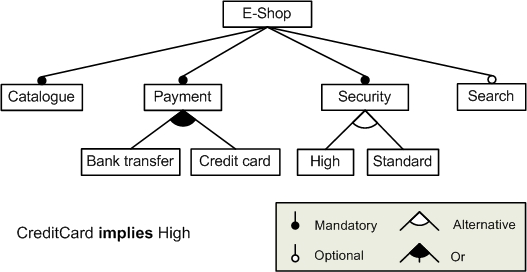
\includegraphics[width=0.7\textwidth]{diagramma.png}
\caption{\textit{Feature Diagram} per un sistema di Shopping Online.}
\label{fig:diagramma}
\end{figure}
\end{mdframed}


\section{Indicatori di variabilità}  % tipi di ambiguità e indicatori dei tipi di ambiguità
\label{sec:indicatori}
Come già discusso in \cref{sec:spl}, i difetti di ambiguità nei requisiti, possono fornire un'indicazione di variabilità (relativa al design, alle scelte implementative o agli aspetti di configurabilità).

\begin{mdframed}
\small
La \textsf{Variabilità} in un requisito rappresenta la \textit{capacità} del requisito stesso di corrispondere a più di una possibile configurazione e di essere modificato o esteso a seconda del contesto specifico in cui viene implementato.
\end{mdframed}

In \cite{oai:it.cnr:prodotti:424687,oai:it.cnr:prodotti:474934,oai:it.cnr:prodotti:458001}, si propone una classificazione dei difetti di ambiguità che possono indicare la presenza di variabilità nei requisiti\footnote{L’analisi fornita è pensata per un testo scritto in lingua inglese.}, facilitando così l'analisi e la gestione della stessa all'interno del processo di sviluppo delle linee di prodotto software.


\subsubsection{\textsf{Vaghezza}}
Il requisito contiene parole che non hanno un significato quantificabile univoco come: \textit{acceptable}, \textit{bad}, \textit{clear}, \textit{clearly}, \textit{difficult}, \textit{easy}, \textit{good}, \textit{hard}, \textit{important}, \textit{inefficient}, \textit{irrelevant}, \textit{significant}, \textit{simple}, \textit{strong} e \textit{unfair}.


\subsubsection{\textsf{Debolezza}}
Il requisito contiene un verbo \textit{debole} che rende la frase non-imperativa. Termini che indicano soggettività includono \textit{can}, \textit{could} e \textit{may}. I casi di debolezza sono direttamente classificabili come variabilità quando introducono una scelta nella configurazione del sistema o una opzionalità in una \textit{feature}.


\subsubsection{\textsf{Forma passiva}}
Una frase in forma passiva è considerata ambigua se non ci sono indicazioni dell'agente che compie l'azione (mancanza della preposizione \textit{by}). Se diverse varianti del prodotto sono previste per i differenti agenti che compiono l'azione, potrebbe esserci un punto di variabilità.


\subsubsection{\textsf{Opzionalità}}
% Il requisito contiene una parte opzionale (che può essere omessa). \torevise{Il requisito contiene un esplicito indicatore di opzionalità. Termini che possono essere indicatori di opzionalità sono:} Termini che in questo caso identificano l'opzionalità sono: \textit{eventually}, \textit{if} \textit{needed}, \textit{optionally}, \textit{possibly} e \textit{probably}. L'opzionalità è direttamente classificabile come una variabilità quando introduce una possibile scelta nella configurazione del sistema.
Il requisito contiene un esplicito indicatore di opzionalità. Termini che possono essere indicatori di opzionalità sono: \textit{eventually}, \textit{if} \textit{needed}, \textit{optionally}, \textit{possibly} e \textit{probably}. L'opzionalità è direttamente classificabile come una variabilità quando introduce una possibile scelta nella configurazione del sistema.


\subsubsection{\textsf{Molteplicità}}
% Il requisito non si riferisce a un singolo oggetto ma si rivolge a più oggetti, tipicamente usando disgiunzioni quali \textit{and}, \textit{or} e \textit{and/or}. In particolare, per disgiunzioni di frasi nominali (NP-molteplicità) è probabile che il requisito evidenzi una \torevise{disgiunzione tra features.} intera gamma di \textit{features}.
Il requisito non si riferisce a un singolo oggetto ma si rivolge a più oggetti, tipicamente usando disgiunzioni quali \textit{and}, \textit{or} e \textit{and/or}. In particolare, per disgiunzioni di frasi nominali (NP-molteplicità) è probabile che il requisito evidenzi una disgiunzione tra \textit{features}.


\subsubsection{\textsf{If, when, where}}
Questi sono casi di clausole subordinate che, oltre a contenere le suddette congiunzioni, presentano anche un verbo come \textit{available}, \textit{provided} e \textit{implemented}.


\subsection{Caso di studio: \textsf{Coffee Vending-Machine}}
% \torevise{Tutta la sezione 2.2, che motiva l'intero lavoro, potrebbe essere curata un pochino di più, in modo da far capire in modo semplice al lettore la corrispondenza tra queste classi di indicatori e i punti di variabilità. Magari con degli esempi presi dai nostri articoli}
Lo scopo di questa sezione è quella di fornire un esempio pratico nel quale l'analisi della variabilità viene condotta attraverso un'attenta disamina dei requisiti espressi. Come evidenziato in \cite{oai:it.cnr:prodotti:474934}, il caso di studio espone la metodologia di identificazione della variabilità a partire da potenziali ambiguità nei requisiti.

\begin{mdframed}
\small
Consideriamo i seguenti requisiti per una \textsf{Coffee Vending-Machine}:
\begin{itemize}[itemsep=0pt]
\item[\textbf{R1.}] After inserting a suitable coin, the user shall choose a beverage and select the amount of sugar.
\item[\textbf{R2.}] The machine shall offer, as beverages, coffee and cappuccino or tea.
\item[\textbf{R3.}] The machine shall always offer coffee.
\item[\textbf{R4.}] A ringtone possibly has to be played after beverage delivery.
\item[\textbf{R5.}] After the beverage is taken, the machine returns idle.
\item[\textbf{R6.}] The British market requires tea and excludes any ring tone.
\end{itemize}
\end{mdframed}

Nel requisito \textbf{R1} si parla di inserire una moneta valida (\textit{suitable coin}): questa \textsf{vaghezza} è un indicatore di variabilità poichè la macchina potrebbe essere configurata per accettare diverse valute. Essa può essere rappresentata con una scelta nel diagramma delle \textit{features}.

Il requisito \textbf{R2} contiene le disgiunzioni \textit{and} e \textit{or}, indicando che la macchina potrebbe offrire caffè e cappuccino o tè. La frase del requisito successivo tuttavia, afferma che il caffè debba essere sempre offerto, indicando la presenza di una \textit{feature} obbligatoria. Questo requisito è un esempio di \textsf{molteplicità} che può essere rappresentata con una disgiunzione nel diagramma delle \textit{features}.

Il requisito \textbf{R4} specifica che un avviso sonoro potrebbe seguire la consegna di una bevanda (\textit{a ringtone possibly has to be played}), indicando questa come una \textit{feature} opzionale della macchina.

\begin{figure}[H]
\centering
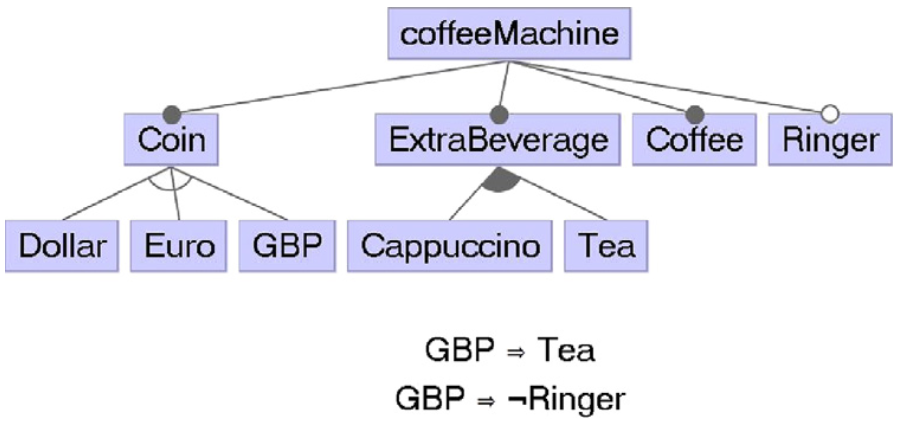
\includegraphics[width=0.7\textwidth]{coffee.png}
\caption{\textit{Feature Diagram} per il caso di studio \textsf{Coffee Vending-Machine}.}
\label{fig:coffee}
\end{figure}

Nei requisiti forniti sono identificabili due vincoli di \textit{inter-feature}\footnote{Un requisito può indicare alcuni vincoli che esprimono implicazioni o relazioni di mutua esclusione tra \textit{features}. Gli indicatori sono termini come \textit{imply}, \textit{require}, \textit{entail}, \textit{implicate}, \textit{demand}, \textit{exclude}, \textit{rule out}, \textit{mutually}, \textit{exclusive} e \textit{need}.}: a questo proposito \textbf{R6} introduce un vincolo per il mercato britannico, escludendo l'avviso sonoro e rendendo obbligatorio il tè.


% PAGINA BIANCA
\clearpage\thispagestyle{empty}
\null\newpage




% CAPITOLO 3
\chapter{\nlp \& \spacy}
\label{ch:nlp}
% Il \textit{Natural Language Processing} (\nlp) rappresenta un ramo dell'Intelligenza Artificiale \torevise{non solo AI: se fai analisi lessicale cercando termini per esempio sei di molto deterministico (e infatti poi lo dici)} focalizzato su l'analisi, la comprensione e la generazione del linguaggio umano attraverso metodi computazionali. Le tecniche di \nlp si avvalgono sia di metodi, quali rappresentazione linguistica e algoritmica classica, che tecniche più moderne legate all'apprendimento automatico.
Il \textit{Natural Language Processing} (NLP) costituisce un campo interdisciplinare al crocevia tra linguistica computazionale, scienza del linguaggio e intelligenza artificiale, che si concentra sull'analisi, la comprensione e la generazione del linguaggio umano mediante metodi computazionali. Le tecniche di NLP spaziano dall'analisi lessicale e algoritmi deterministici basati su regole, fino a metodologie più moderne che sfruttano l'apprendimento automatico e le reti neurali.

Dato un testo, l'elaborazione del linguaggio naturale prevede diverse fasi per analizzarlo e comprenderlo:

\begin{enumerate}
\item \textsf{Tokenizzazione} -- Fase iniziale di analisi lessicale in cui il testo viene suddiviso in unità significative chiamate token: questi possono rappresentare parole o frasi e forniscono la base per le successive elaborazioni.
\item \textsf{Analisi morfologica} -- Questa fase si occupa di identificare il ruolo di ogni token\footnote{Come mostrato in \cref{sec:tokenizzazione}, i token sono etichettati con le informazioni qua ottenute.} nel discorso (nomi, verbi, aggettivi e altri elementi grammaticali) e di analizzare la struttura delle parole per identificarne prefissi, suffissi e radici. Permette inoltre di estrarre la forma base di una parola (\cref{sec:lemmatizzazione}) o la sua \textit{categoria grammaticale}\footnote{Una \textit{categoria grammaticale} si riferisce alla funzione che una parola svolge nella frase in base alla sua morfologia e sintassi. Le categorie grammaticali sono classificate principalmente in parti del discorso: sostantivi, verbi, aggettivi, avverbi, pronomi, preposizioni, congiunzioni e interiezioni. Ogni categoria possiede regole specifiche relative a flessione, concordanza e costruzione frasale. Per esempio, i sostantivi possono essere classificati in base al genere (maschile, femminile, neutro), al numero (singolare, plurale) e al caso (nominativo, genitivo, dativo \dots), mentre i verbi si coniugano a seconda del tempo, modo, aspetto e voce.}.
\item \textsf{Analisi sintattica} -- Studia la struttura grammaticale delle frasi e le relazioni di dipendenza tra i token: analizza come le parole si combinano tra loro per creare un significato. Questo permette di identificare soggetto, verbo, complemento e altre parti del discorso all'interno di una frase.
\item \textsf{Analisi semantica} -- Qui l'attenzione si concentra sul significato delle frasi in riferimento al contesto dato. Questa fase cerca di interpretare il significato delle parole e delle frasi in base al contesto in cui vengono utilizzate, come ad esempio l'identificazione di sinonimi o l'interpretazione di espressioni idiomatiche.
\end{enumerate}


\section{L'ecosistema \spacy}
Nel panorama degli strumenti per il \textit{Natural Language Processing}, \spacy si distingue per la sua progettazione orientata alla produzione e per le prestazioni di alto livello. Come libreria open-source di \nlp, \spacy offre un'architettura robusta e ottimizzata, focalizzata sulla velocità e sull'accuratezza, che la rende una scelta privilegiata per l'implementazione in applicazioni di scala industriale.

La peculiarità di \spacy risiede nel suo approccio pragmatico alla risoluzione di problemi di \nlp: la libreria è stata progettata per essere utilizzata in contesti reali, dove la necessità di affidabilità ed efficienza è prioritaria. Ciò si traduce in una suite di algoritmi e modelli linguistici pre-addestrati su vasti \textit{corpora di testo}\footnote{Il termine \textit{corpora di testo} si riferisce a raccolte di testi scritti o trascritti, organizzati sistematicamente e utilizzati come base per la ricerca nel campo della linguistica, della traduzione e, più recentemente, nell'elaborazione del linguaggio naturale. Un \textit{corpus} è spesso annotato linguisticamente: questo significa che è stato marcato per fornire informazioni aggiuntive di tipo grammaticale, sintattico e semantico.\\
Nel contesto di \spacy, i \textit{corpora di testo} sono utilizzati per addestrare modelli statistici che apprendono da esempi reali come riconoscere e interpretare vari aspetti del linguaggio (e.g. struttura delle frasi e significato del contesto). Questi \textit{corpora} possono variare da collezioni generali di testi a dataset di settori altamente specializzati, come quello medico, giuridico o tecnologico. L'uso di \textit{corpora} vasti e variati consente ai modelli di \nlp di essere particolarmente accurati quando poi applicati al linguaggio naturale nel quotidiano.} in lingue diverse.

Uno degli aspetti salienti di \spacy è l'astrazione fornita dalla sua \api, la quale consente al programmatore di implementare rapidamente funzionalità di \nlp senza doversi addentrare nella complessità degli algoritmi sottostanti. Ciò semplifica notevolmente il processo di sviluppo e consente di concentrarsi sull'integrazione e sull'ottimizzazione delle funzionalità di analisi del linguaggio all'interno delle applicazioni.

\spacy permette anche una personalizzazione avanzata, grazie alla possibilità di estendere e adattare i modelli preesistenti o di addestrarne di nuovi: caratteristica particolarmente utile quando si lavora con testi di dominio specifico.

La libreria è inoltre facilmente integrabile con altre piattaforme come \textsl{TensorFlow} e \textsl{PyTorch}, facilitando la creazione di pipeline di elaborazione dati end-to-end.

In conclusione, \spacy rappresenta un ecosistema completo e altamente scalabile per l'analisi del linguaggio naturale, che soddisfa esigenze di ricercatori e sviluppatori, offrendo strumenti performanti e versatili.

Nelle fasi successive saranno mostrate le funzionalità di \spacy, utilizzate per l'implementazione del parser \toody.


\subsection{Tokenizzazione}
\label{sec:tokenizzazione}
Come precedentemente descritto, la \textsf{Tokenizzazione} è il primo passo nell'analisi di un testo in \nlp. \spacy esegue una suddivisione del testo in unità minime, o token, che rappresentano le parole, i simboli di punteggiatura e altri elementi costitutivi del linguaggio.

Il processo di Tokenizzazione in \spacy non si limita a una semplice segmentazione del testo basata su spazi e segni di punteggiatura, ma utilizza un modello complesso che prende in considerazione le regole grammaticali e le eccezioni linguistiche. Questo approccio permette di gestire efficacemente anche le parole composte, le contrazioni e altri casi speciali che possono variare da una lingua all'altra.

Per eseguire la Tokenizzazione, \spacy si avvale di regole morfologiche (eventualmente estensibili) per ciascuna lingua supportata. Vengono usate espressioni regolari e modelli statistici per raffinare ulteriormente il processo di suddivisione del testo, facendo sì che i token generati siano il più possibile precisi e utili per le fasi successive dell'analisi.

Ogni token è un oggetto ricco di attributi, quali:

\begin{itemize}
    \item \textsf{Lemma} -- Forma base o canonica di una parola, utile per il riconoscimento delle diverse \textit{flessioni}\footnote{Qui il termine \textit{flessioni} si riferisce alle \textit{forme flesse} di una parola base (\cref{sec:lemmatizzazione}).} come identiche.
\item \textsf{PoS-Tags} -- Assegnazione di parti del discorso (sostantivi, verbi, aggettivi) che fornisce un contesto sintattico.
\item \textsf{Dipendenze Sintattiche} -- Relazioni di dipendenza tra i token che aiutano a identificare la struttura grammaticale di una frase.
\item \textsf{Flag Morfologici} -- Informazioni sulla morfologia di una parola, quali genere, cardinalità, tempo e caso.
\item \textsf{Entità Riconosciute} -- Entità nominate (persone, luoghi, organizzazioni) che il token può rappresentare.
\item \textsf{Similarità Semantica} -- Misura della somiglianza tra token in termini di significato, basata su modelli vettoriali.
\item \textsf{Shape} -- Rappresentazione della forma della parola che indica se un token è maiuscolo, minuscolo, un numero o una punteggiatura.
\item \textsf{Spazi} -- Segnalazioni della presenza di un carattere bianco dopo il token nel testo originale.
\item \textsf{Flag personalizzati} -- Possibilità di aggiungere attributi personalizzati definiti dall'utente per esigenze specifiche.
\end{itemize}

% \vspace{-0.45cm}
% {\centering \rule{0.5\linewidth}{0.1pt} \par\vspace{0.25cm}}

\begin{mdframed}
\small
Ecco un esempio di Tokenizzazione in \spacy. Viene importata la libreria, caricato il modello linguistico italiano e analizzata una stringa di testo:

\begin{lstlisting}[language=Python]
import spacy

nlp = spacy.load("it_core_news_sm")
testo = "L'analisi del linguaggio naturale è affascinante."
doc = nlp(testo)
tokens = [token.text for token in doc]
\end{lstlisting}

{\centering \rule{0.5\linewidth}{0.1pt} \par\vspace{0.25cm}}

\noindent Il valore della variabile \texttt{tokens} contenente l'elenco completo dei token generati è il seguente:

\begin{lstlisting}[language=Python]
[
    "L'", "analisi", "del", "linguaggio",
    "naturale", "è", "affascinante", "."
]
\end{lstlisting}
\end{mdframed}

\noindent Nell'esempio, \spacy ha correttamente identificato \texttt{"L'"} come un token separato, dimostrando la sua capacità di gestire le contrazioni nella lingua italiana. Inoltre, il \texttt{"."} alla fine della frase è stato riconosciuto come un token indipendente, mostrando come \spacy consideri la punteggiatura parte integrante della struttura del testo.


\subsection{PoS-Tagging}
La procedura di PoS-Tagging (Part-of-Speech tagging), illustra come \spacy, durante la fase di \textsf{Analisi morfologica}, assegni una specifica etichetta (e.g. sostantivo, verbo, aggettivo) a ciascun token\footnote{Dopo la Tokenizzazione del testo, \spacy utilizza i contesti dei token per etichettarli.\\
E.g. In \textit{Il gatto dorme sul divano}, \textit{gatto} e \textit{divano} saranno etichettati come sostantivi (\texttt{NOUN}), mentre \textit{dorme} come verbo (\texttt{VERB}).}: questo passo è importante per comprendere la struttura grammaticale e il significato di una frase, giacché la funzione di una parola in un dato contesto può mutare il significato della stessa o quello dell'intera espressione.

In \spacy, le etichette di Part-of-Speech sono basate su un insieme di convenzioni standard come quelle del \textit{Penn Treebank}\footnote{Il \textit{Penn Treebank} è un famoso progetto sviluppato all'Università della Pennsylvania nei primi anni '90 che ha prodotto una raccolta annotata di materiale testuale incluso etichette di Part-of-Speech: queste sono diventate lo standard-de-facto per il PoS-Tagging in lingua inglese. (E.g. \texttt{NN} per sostantivi singolari, \texttt{VB} per verbi in forma base, \texttt{JJ} per aggettivi).\\
\spacy utilizza un sistema di etichettatura simile a quello del \textit{Penn Treebank} per l'inglese, ma adatta ed estende queste convenzioni per supportare altri linguaggi e fornire una analisi del testo al passo con i tempi. Ciò significa che \spacy non segue le convenzioni del \textit{Penn Treebank} alla lettera, ma si ispira ad esse per creare un sistema di etichettatura che sia coerente, intuitivo e applicabile a più lingue, inclusi aspetti che possono non essere coperti o che si sono evoluti nel tempo, rispetto al progetto originale.} per l'inglese, con alcune personalizzazioni per meglio adattarsi alle esigenze della moderna analisi del testo, oltre che ai diversi linguaggi supportati dalla libreria.

Ogni token in \spacy ha un attributo \texttt{.pos\_} che indica il PoS-Tag semplice e un attributo \texttt{.tag\_} che fornisce il tag dettagliato, specifico del modello linguistico caricato.

La precisione del PoS-Tagging è fondamentale per molte altre funzionalità di \nlp, come l'analisi sintattica e la lemmatizzazione: una etichettatura corretta permette di costruire l'analisi sintattica in maniera accurata e determinare l'esatto lemma di una parola. Inoltre, \spacy offre la possibilità di personalizzare e addestrare ulteriormente i modelli di PoS-Tagging su corpora specifici, permettendo di migliorare ulteriormente l'accuratezza dell'analisi eseguita su domini specializzati o per lingue con risorse limitate.


\subsection{Dependency Parsing}
Il parsing delle dipendenze è una parte specifica dell'\textsf{Analisi sintattica} che si occupa di analizzare la struttura grammaticale di una frase e di stabilire le relazioni di dipendenza tra le parole, ovvero come ogni parola dipenda da un'altra all'interno della frase. In \spacy, il Dependency Parsing è un processo fondamentale che permette di comprendere la struttura sintattica delle frasi e di identificare le relazioni gerarchiche tra le parole.

Dopo i processi di Tokenizzazione e PoS-Tagging, \spacy utilizza il Dependency Parsing per generare un albero delle dipendenze che rappresenta la struttura sintattica dei token in una frase\footnote{\spacy impiega modelli addestrati su corpora di testo annotati che contengono informazioni sulle relazioni sintattiche: questi modelli utilizzano algoritmi di apprendimento automatico per prevedere le dipendenze, basandosi sul contesto e sulla funzione grammaticale delle parole.}. Il token radice è chiamato \textit{head} ed è tipicamente il verbo principale dal quale dipendono tutte le altre parole della frase; i token subordinati sono denominati \textit{children}.

Ogni arco dell'albero delle dipendenze ha un'etichetta che indica il tipo di relazione (ruolo sintattico) tra il token \textit{head} e il token \textit{children}\footnote{Esempi di etichette sono: \texttt{nsubj} (soggetto nominale), \texttt{dobj} (oggetto diretto), \texttt{advmod} (modificatore avverbiale).}.

% {\centering \rule{0.5\linewidth}{0.1pt} \par\vspace{0.25cm}}

\begin{mdframed}
\small
Prendiamo come esempio la frase \textit{Il gatto mangia il cibo.} \spacy eseguirà Tokenizzazione e PoS-Tagging, identificando \textit{gatto} come sostantivo e \textit{mangia} come verbo. Con il Dependency Parsing, \spacy costruirà poi un albero in cui \textit{mangia} rappresenterà il token radice, mentre \textit{gatto} e \textit{cibo} saranno etichettati rispettivamente come \texttt{nsubj} (soggetto nominale di \textit{mangia}) e \texttt{obj} (oggetto di \textit{mangia}).

Questo mostra come \textit{gatto} e \textit{cibo} siano collegati dal verbo \textit{mangia}, stabilendo una chiara struttura grammaticale della frase.
\end{mdframed}


\subsection{Lemmatizzazione}
\label{sec:lemmatizzazione}
La lemmatizzazione è parte dell'\textsf{Analisi morfologica} nell'elaborazione del linguaggio naturale che riduce le parole al loro \textit{lemma}\footnote{Il \textit{lemma} è la forma base di una parola, da cui derivano tutte le altre forme flesse.\\
Se analizziamo la parola \textit{correndo}, essa è la forma del verbo \textit{correre} al gerundio presente. La forma base di un verbo in lingua italiana è quella coniugata al tempo infinito, quindi in questo caso \textit{correre}.\\
Se analizziamo la parola \textit{corsa}, essa è la forma nominale (quella indicante il nome dell'azione o dello stato espresso) del verbo \textit{correre} e in questo caso, \textit{corsa} indica l'azione di correre, quindi la forma base sarà sempre \textit{correre}.\label{fn:lemma}}.

In \spacy, la lemmatizzazione inizia con l'identificazione della parte del discorso di un token: questa informazione è da considerarsi cruciale poiché la forma base di una parola può variare a seconda della sua funzione grammaticale\footnote{\textit{ancora} potrebbe essere usata come avverbio di tempo, come in \textit{Sto ancora lavorando}, nella quale il lemma è la parola stassa \textit{ancora}. Tuttavia, \textit{ancora} potrebbe essere un sostantivo, come in \textit{L'ancora della nave è pesante}, dove il lemma è nuovamente \textit{ancora}.}.

Per le lingue come l'inglese, che presentano un numero limitato di forme flesse, le regole morfologiche possono essere sufficienti per una lemmatizzazione accurata. Tuttavia, per lingue morfologicamente più complesse \spacy utilizza modelli statistici. Questi modelli sono addestrati su ampi corpora di testo annotati manualmente, dove le forme base delle parole sono già state identificate\footnote{La combinazione di regole morfologiche e modelli statistici rende il processo di lemmatizzazione in \spacy particolarmente efficace, oltre al fatto che gli utenti hanno la possibilità di personalizzare ed estendere le regole di lemmatizzazione o di aggiungere le proprie, per lingue e contesti specifici.}. Attraverso l'apprendimento automatico, \spacy impara a riconoscere pattern nei dati e ad applicare questa conoscenza alla lemmatizzazione di nuovi input di testo.

L'oggetto \texttt{Token} in \spacy offre una proprietà \texttt{.lemma\_} che restituisce il lemma di un token: questo attributo è particolarmente utile nell'elaborazione del linguaggio, come nella normalizzazione del testo per compiti di classificazione o ricerca; ciò permette di concentrarsi sul significato piuttosto che sulla forma esteriore.


\subsection{Sentence Boundary Detection}
In \spacy, la Sentence Boundary Detection identifica i confini tra frasi all'interno di un testo: questa funzione non è menzionata esplicitamente nelle fasi di analisi in \nlp, ma è implicita nella \textsf{Tokenizzazione} e nell’\textsf{Analisi sintattica}.

La Sentence Boundary Detection è tipicamente gestita dal parser e, come le precedenti funzioni, fa uso di modelli statistici e di apprendimento automatico. Questi modelli sono stati addestrati su ampi corpora di testo e sono in grado di riconoscere i segnali tipici che indicano la fine di una frase, quali punto, punto esclamativo, punto interrogativo, nuova linea e pause. Analizzando la struttura della frase fatta dal Dependency Parsing, \spacy distingue quando la punteggiatura non corrisponde alla fine di una frase come nel caso di abbreviazioni e acronimi\footnote{Si consideri il seguente testo: \textit{Dr. Rossi lavora all'ospedale. È un cardiologo rinomato.} \spacy riconosce che \textit{Dr.} non segnala la fine di una frase ma è seguito da una nuova frase.\\
In generale, anche in altre situazioni nelle quali la punteggiatura può essere ambigua o mancante (e.g. dialoghi trascritti o testo parlato) e i segnali di terminazione di frase possono essere meno evidenti, \spacy si avvale del contesto per determinare i limiti delle frasi.}.

Inoltre, in testi con un particolare stile o genere (come quello letterario, dove i confini delle frasi sono meno standard), \spacy dà la possibilità di personalizzare la Sentence Boundary Detection aggiungendo regole specifiche o modificando il modello per meglio adattarsi alla situazione.


\subsection{Named Entity Recognition}
Durante la fase di \textsf{Analisi semantica}, \spacy esegue il processo di Named Entity Recognition per identificare e classificare elementi del testo in categorie predefinite come nomi di persone, organizzazioni, località, espressioni di tempo, quantità, valute, date e altre entità nominate.

Questo processo, come i precedenti, è realizzato attraverso modelli statistici addestrati su corpora di testo annotati: questo consente il riconoscimento di schemi e indicatori linguistici che suggeriscono la presenza delle entità. Dopo \textsf{Tokenizzazione}, \textsf{Analisi morfologica} e \textsf{Analisi sintattica}, \spacy  esamina ciascun token e relativo contesto per dedurre l'appartenenza a una delle categorie riconosciute e lo etichetta con il tipo corrispondente\footnote{Si consideri la seguente frase: \textit{Leonardo da Vinci nacque ad Anchiano}. \spacy riconosce \textit{Leonardo da Vinci} come \texttt{PERSON} (persona) e \textit{Anchiano} come \texttt{LOC} (località).\\
La libreria è anche capace di gestire entità composte da più token (e.g. \textit{Regno Unito} e \textit{Torre Eiffel}), assicurandosi che l'intera espressione venga identificata come entità unica.}.

Per il riconoscimento di termini tecnici o di forme gergali, gli sviluppatori possono addestrare i propri modelli su corpora personalizzati o aggiungere nuove categorie di entità per incrementare la copertura e l’accuratezza del riconoscimento.


\subsection{Rule-Based Matching}
Questa funzionalità dell'\textsf{Analisi sintattica} consente di identificare ed estrarre sequenze di token basate su modelli di regole specifici definite dal programmatore. Questo strumento è particolarmente utile per quei casi in cui le espressioni regolari sono troppo limitanti e dove è necessario un approccio più raffinato che possa tenere conto del contesto linguistico, come le categorie grammaticali identificate dal PoS-Tagging e la struttura sintattica delle parole generata dal Dependency Parsing.

\spacy implementa il Rule-Based Matching tramite il componente \texttt{Matcher}, che permette di costruire modelli di regole complessi utilizzando le proprietà dei token, quali testo, lemma, PoS e relazioni di dipendenza sintattica.

Il funzionamento ha inizio con la definizione di pattern, ciascuno rappresentato come una lista di dizionari che definiscono le caratteristiche dei token; questi vengono aggiunti al \texttt{Matcher} che li utilizza per scansionare il documento.

Il \texttt{Matcher} restituirà un insieme di \textit{match}\footnote{Ciascun \textit{match} corrisponde a una tupla contenente: identificativo del match, indice di inizio e indice di fine sequenza.} ogni qualvolta trova una corrispondenza tra il pattern e una sequenza di token nel documento.

\begin{mdframed}
\small
Ecco un esempio di Rule-Based Matching in \spacy con l'oggetto \texttt{Matcher}. Viene definito un pattern per identificare aggettivi seguiti da un nome:

\begin{lstlisting}[language=Python]
import spacy
from spacy.matcher import Matcher

nlp = spacy.load("it_core_news_sm")
matcher = Matcher(nlp.vocab)
pattern = [{"POS": "NOUN"}, {"POS": "ADJ"}]
matcher.add("NOUN_ADJ_PATTERN", [pattern])

doc = nlp(
    "Il mercato azionario ha mostrato"
    "una crescita costante."
)

matches = matcher(doc)
\end{lstlisting}
\end{mdframed}


\begin{mdframed}
\small
Per visualizzare i match trovati nel documento, si può aggiungere un ciclo che percorra \texttt{matches} e stampi il testo corrispondente da \texttt{doc}, utilizzando gli indici di inizio e fine \texttt{start} e \texttt{end}:

\begin{lstlisting}[language=Python]
for match_id, start, end in matches:
    matched_span = doc[start:end]
    print(matched_span.text)
\end{lstlisting}

{\centering \rule{0.5\linewidth}{0.1pt} \par\vspace{0.25cm}}

\noindent I match stampati saranno dunque:

\begin{lstlisting}
mercato azionario
crescita costante
\end{lstlisting}
\end{mdframed}

Esistono altri componenti in \spacy simili a \texttt{Matcher} che permettono di eseguire il Rule-Based Matching per casi specifici: \texttt{PhraseMatcher} (per l'identificazione di frasi) che sarà utile per l'implementazione del parser di \toody e \texttt{DependencyMatcher} (per identificare relazioni di dipendenza sintattica). Ciascuno di essi ha un approccio diverso per la definizione dei pattern.


\subsubsection{PhraseMatcher}
Come anticipato, \texttt{PhraseMatcher} è un componente di \spacy che, analogamente a \texttt{Matcher}, serve per trovare sequenze di parole o frasi all'interno di un documento. Tuttavia, a differenza di \texttt{Matcher} che cerca token basandosi su pattern di attributi, \texttt{PhraseMatcher} individua occorrenze di frasi specifiche.

Esso è particolarmente utile per il matching esatto e veloce di grandi liste di termini, come nel caso di applicazioni per l'estrazione di entità nominate o per il riconoscimento di termini tecnici.

\texttt{PhraseMatcher} si differenzia da \texttt{Matcher} per i seguenti punti:

\begin{enumerate}
\item \textsf{Ricerca basata su termini esatti} -- Mentre \texttt{Matcher} può cercare token che soddisfano criteri generali o basati su pattern, \texttt{PhraseMatcher} individua specifiche stringhe di testo. Questo lo rende più adatto al riconoscimento di frasi definite in modo esatto all'interno del testo.
\item \textsf{Efficienza con grandi liste di termini} -- Grazie alla sua implementazione, \texttt{PhraseMatcher} è molto efficiente nella ricerca di un gran numero di frasi. Questo lo rende ideale per il matching di frasi in corpora di testo di grandi dimensioni.
\item \textsf{Uso di \texttt{Doc} objects} -- A differenza di \texttt{Matcher} che utilizza pattern rappresentati come liste di dizionari, \texttt{PhraseMatcher} impiega oggetti \texttt{Doc} per la definizione dei sui pattern. Ogni frase da cercare viene elaborata dall'oggetto \texttt{nlp}\footnote{L'oggetto \texttt{nlp} è alla base dell'elaborazione del testo con \spacy. \texttt{nlp} viene creato caricando un modello linguistico che contiene la pipeline di elaborazione del linguaggio e vari asset come vocabolario, patterns e modelli statistici.} che restituirà un oggetto \texttt{Doc}, utilizzato poi come pattern di ricerca.
\end{enumerate}


\begin{mdframed}
\small
Ecco un esempio di utilizzo: \texttt{PhraseMatcher} trova le occorrenze delle frasi \textit{intelligenza artificiale} e \textit{realtà virtuale} all'interno di una stringa di testo. Trovato un match, viene stampato il testo corrispondente:

\begin{lstlisting}[language=Python]
import spacy
from spacy.matcher import PhraseMatcher

nlp = spacy.load("it_core_news_sm")

# creazione oggetto PhraseMatcher
phrase_matcher = PhraseMatcher(nlp.vocab)

# definizione pattern
phrases = ["intelligenza artificiale", "realtà virtuale"]
patterns = [nlp(text) for text in phrases]
phrase_matcher.add("TECH_PATTERNS", patterns)

doc = nlp(
    "L'intelligenza artificiale e la realtà virtuale "
    "sono due delle tecnologie più innovative."
)

# ricerca dei pattern nel documento
matches = phrase_matcher(doc)

for match_id, start, end in matches:
    matched_span = doc[start:end]
    print(matched_span.text)
\end{lstlisting}
\end{mdframed}


% PAGINA BIANCA
\clearpage\thispagestyle{empty}
\null\newpage




% CAPITOLO 4
\chapter{\toody analyzer}
\label{ch:parser}
% In questo capitolo verranno presentati i diversi algoritmi che compongono il parser dell'analisi \torevise{il parser dell'analisi non è chiaro, scrivi meglio: In questo capitolo verranno presentati le diverse componenti di \toody che permettono di fare un parsing lessicale e sintattico per identificare...} del testo e che permettono a \toody di identificare i punti variabilità nei documenti dei requisiti.
In questo capitolo verranno presentati le diverse componenti di \toody che permettono di fare un parsing lessicale e sintattico per identificare i punti variabilità nei documenti dei requisiti.

L'analisi effettuata si basa sui principi definiti nella \cref{sec:indicatori}, nella quale sono delineate una serie di caratteristiche linguistiche che suggeriscono la presenza di variabilità nei requisiti. Tra queste si ricordano: uso di termini vaghi e opzionali, forme passive e specifiche costruzioni sintattiche con congiunzioni (\textit{if}, \textit{when}, \textit{where}).

Per raggiungere questo obiettivo, vengono impiegate una combinazione di tecniche di elaborazione del linguaggio naturale fornite dalla libreria \spacy, per rilevare e interpretare queste caratteristiche nei testi analizzati.


\section{Implementazione parser}
Nel contesto del progetto \toody, sfruttando la potenza e la versatilità della libreria \spacy, sono state sviluppate quattro funzioni specializzate che offrono un'analisi completa dei documenti dei requisiti\footnote{L'analisi fornita è pensata per un testo scritto in lingua inglese.}. Queste sono integrate all'interno del server realizzato in \flask e hanno il compito di processare e analizzare il testo dei requisiti inviato dal client, offrendo un'interpretazione dettagliata e accurata dei vari aspetti linguistici contenuti nei documenti.

Il \textsf{parser lessicale} è progettato per analizzare i documenti di requisiti e identificare specifici pattern linguistici. Questo parser suddivide il testo in token, e con l'aiuto di un \texttt{PhraseMatcher}, cerca frasi o termini predefiniti all'interno del documento. Ogni corrispondenza trovata viene classificata e annotata, fornendo una panoramica dettagliata delle occorrenze e del loro contesto nel documento.

Il \textsf{parser di forma passiva} si focalizza sull'identificazione delle frasi che non specificano il complemento di agente, spesso fonte di ambiguità nei documenti dei requisiti. Analizza la struttura grammaticale di ogni frase per rilevare verbi al participio passato usati con ausiliari passivi (come \textit{be}), escludendo le strutture con un agente esplicito (\textit{by}).

Il \textsf{parser di congiunzioni verbali} identifica e analizza l'uso di specifiche congiunzioni (come \textit{when}, \textit{where}, \textit{if}) in relazione a specifici verbi all'interno del documento in argomento. Questo strumento si concentra su verbi target come \textit{provide} o \textit{modified}, cercando le loro associazioni con congiunzioni che indicano condizioni. Tale analisi è vitale per capire come determinate azioni o condizioni influenzino le funzionalità descritte nei requisiti, migliorando la comprensione delle dipendenze funzionali.

L'\textsf{analizzatore di disgiunzioni} si focalizza sull'identificazione e analisi dell'uso di congiunzioni specifiche (\textit{or}, \textit{and/or}) tra le frasi del documento dei requisiti. Questa funzione esamina come le congiunzioni colleghino elementi nominali, catturando la relazione tra diversi componenti o condizioni. Tale analisi risulta utile a comprendere le scelte alternative o combinate presenti nei requisiti, fornendo informazioni sulla struttura logica e le opzioni disponibili nel testo.


\subsection{Parser lessicale}
\label{subsec:parser_lessicale}
% Analizziamo in dettaglio il codice del \textsf{parser lessicale}.

\begin{mdframed}
\small
\begin{lstlisting}[language=Python]
def lexical_analyser(
    doc_requisiti,
    content1,
    content2,
    lexical_memory
):
\end{lstlisting}
\end{mdframed}

\noindent La funzione prende quattro parametri: \texttt{doc\_requisiti} che rappresenta il doc-object del documento dei requisiti da analizzare, \texttt{content1} e \texttt{content2} che rappresentano rispettivamente il testo del documento dei requisiti e il diziorario dei termini da cercare e \texttt{lexical\_memory} che è una struttura dati necessaria per tenere traccia delle parole già etichettate dal client\footnote{Anticipiamo qua una funzionalità di \toody: il fruitore della web-app ha la possibilità di etichettare manualmente i match trovati dall'algoritmo di ricerca. Il client invierà quindi i match etichettati in modo che il server possa riconoscerli e rispettare le etichettature già effettuate.}.


\begin{mdframed}
\small
\begin{lstlisting}[language=Python]
lexical_patterns = [
    nlp.make_doc(text.strip())
    for text in content2.splitlines()
    if not text.strip().startswith("#")
    and text.strip() != ""
]
\end{lstlisting}
\end{mdframed}

\noindent Questo frammento crea una lista di pattern lessicali necessari per il matcher. Ogni riga in \texttt{content2}, non commentata e non vuota, viene trasformata in documento \spacy (tramite \texttt{nlp.make\_doc}).


\begin{mdframed}
\small
\begin{lstlisting}[language=Python]
matcher = PhraseMatcher(nlp.vocab, attr="LOWER")
matcher.add("LEXICAL_PATTERNS", lexical_patterns)
matches = matcher(doc_requisiti)
\end{lstlisting}
\end{mdframed}

\noindent Qui viene istanziato un oggetto \texttt{PhraseMatcher} (specificando il vocabolario \spacy \texttt{nlp.vocab}) che utilizza i pattern lessicali creati in precedenza. Questo oggetto viene utilizzato per cercare i pattern all'interno del documento dei requisiti.


\begin{mdframed}
\small
\begin{lstlisting}[language=Python]
results = {}
for match_id, start, end in matches:
    span = doc_requisiti[start:end]
    line_number = content1.count(
        "\n", 0, span.start_char
    ) + 1  # continua for
\end{lstlisting}
\end{mdframed}

\noindent Si inizializza un dizionario vuoto per memorizzare i risultati dell'analisi lessicale. Per ogni match trovato, viene estratto il segmento corrispondente (\texttt{span}) dal documento dei requisiti e determinato il numero di riga del match in \texttt{content1}, contando le new-line fino all'inizio di \texttt{span}.


\begin{mdframed}
\small
\begin{lstlisting}[language=Python]
sentence_start = span.sent.start_char
highlighted_sentence = highlight_specific_instance(
    span.sent.text,
    span.text,
    span.start_char - sentence_start,
    span.end_char - sentence_start,
)
highlighted_sentence = highlighted_sentence.replace(
    "\r", ""
)  # continua for
\end{lstlisting}
\end{mdframed}

\noindent Per ogni match, viene evidenziata l'istanza specifica nel contesto della frase, calcolato l'inizio della frase (\texttt{sentence\_start}) ed evidenziato il testo corrispondente\footnote{Qui si aggiunge il marcatore \html che il client userà per evidenziare la parola.}. Vengono rimossi eventuali caratteri di \texttt{<CR>}.


\begin{mdframed}
\small
\begin{lstlisting}[language=Python]
tag = "neutral"
if span.text in lexical_memory:
    for label, sentences in lexical_memory[span.text].items():
        if highlighted_sentence in sentences:
            tag = label
            break

if span.text not in results:
    results[span.text] = []

results[span.text].append({
    "line": line_number,
    "sentence": highlighted_sentence,
    "tag": tag
})  # fine for
\end{lstlisting}
\end{mdframed}

\noindent Viene assegnata un'etichetta predefinita (\texttt{neutral}) ed effettuata una ricerca nella \texttt{lexical\_memory} per controllare se la frase evidenziata sia già classificata, aggiornando eventualmente l'etichetta.

Successivamente si aggiungono le informazioni raccolte (riga, frase evidenziata, etichetta) al dizionario dei risultati.


\begin{mdframed}
\small
\begin{lstlisting}[language=Python]
results = dict(sorted(results.items()))
return results
\end{lstlisting}
\end{mdframed}

\noindent I risultati vengono ordinati alfanumericamente e restituiti.

{\centering \rule{0.5\linewidth}{0.1pt} \par\vspace{0.25cm}}

In sintesi, il processo eseguito dal \textsf{parser lessicale} aiuta a identificare e analizzare in modo dettagliato l’uso di parole chiave all’interno del testo.


\subsection{Parser di forma passiva}
\label{subsec:parser_forma_passiva}
% Analizziamo in dettaglio il codice del \textsf{parser di forma passiva}.

\begin{mdframed}
\small
\begin{lstlisting}[language=Python]
def passive_form_parser(
    doc_requisiti,
    content1,
    passive_memory
):
\end{lstlisting}
\end{mdframed}

\noindent La funzione accetta tre parametri: \texttt{doc\_requisiti} che rappresenta il doc-object del documento dei requisiti da analizzzare, \texttt{content1} che definisce il testo del documento dei requisiti e \texttt{passive\_memory}, struttura usata per memorizzare le frasi passive identificate.


\begin{mdframed}
\small
\begin{lstlisting}[language=Python]
verbs = [
    token
    for token in doc_requisiti
    if (
        token.pos == VERB
        and token.morph.get("VerbForm") == ["Part"]
        and any(
            child.lemma_ == "be" and child.dep_ == "auxpass"
            for child in token.children
        )
\end{lstlisting}
\end{mdframed}


\begin{mdframed}
\small
\begin{lstlisting}[language=Python]
        and not any(
            child.text == "by" and child.dep_ == "agent"
            for child in token.children
        )
    )
]
\end{lstlisting}
\end{mdframed}

\noindent Questo blocco di codice crea una lista di token che rappresenta verbi del documento \texttt{doc\_requisiti}. Vengono considerati tutti quei verbi presenti all'interno di una struttura passiva al participio passato (\texttt{Part}) e hanno \textit{be} in funzione di ausiliare passivo (\texttt{auxpass}); vengono esclusi tutti quelli che hanno un agente espresso da \textit{by}.


\begin{mdframed}
\small
\begin{lstlisting}[language=Python]
sentences = [token.sent for token in verbs]
results = {}
\end{lstlisting}
\end{mdframed}

\noindent Per ogni verbo identificato come passivo, viene estratta la frase corrispondente. Poi si inizializza un dizionario vuoto per i risultati.


\begin{mdframed}
\small
\begin{lstlisting}[language=Python]
for verb, sentence in zip(verbs, sentences):
    sentence_start = sentence.start_char
    highlighted = highlight_specific_instance(
        sentence.text,
        verb.text,
        verb.idx - sentence_start,
        verb.idx - sentence_start + len(verb.text),
    )
    highlighted = highlighted.replace(
        "\r", ""
    )
    # continua for
\end{lstlisting}
\end{mdframed}

\noindent Per ogni verbo, viene evidenziata la sua presenza all'interno della frase. Si calcola l'indice di inizio della frase e si evidenzia il verbo con la funzione \texttt{highlight\_specific\_instance}. Vengono rimossi caratteri di \texttt{<CR>}.


\begin{mdframed}
\small
\begin{lstlisting}[language=Python]
tag = "neutral"
if str(verb) in passive_memory:
    for label, sentences in passive_memory[
        str(verb)
    ].items():
        if highlighted in sentences:
            tag = label
            break
# continua for
\end{lstlisting}
\end{mdframed}

\noindent In questo frammento viene assegnata un'etichetta predefinita (\texttt{neutral}) ed effettuata una ricerca nella \texttt{passive\_memory} per controllare se la frase evidenziata sia già stata classificata in precedenza, aggiornando eventualmente l'etichetta.


\begin{mdframed}
\small
\begin{lstlisting}[language=Python]
line_number = content1.count(
    "\n", 0, sentence.start_char
) + 1
if str(verb) not in results:
    results[str(verb)] = []
results[str(verb)].append({
    "line": line_number,
    "sentence": highlighted_sentence,
    "tag": tag
})
# fine for
\end{lstlisting}
\end{mdframed}

\noindent Qui viene calcolato il numero di riga della frase all'interno di \texttt{content1}. Si aggiungono i dettagli trovati (numero di riga, frase evidenziata, etichetta) al dizionario dei risultati.


\begin{mdframed}
\small
\begin{lstlisting}[language=Python]
results = dict(sorted(results.items()))
return results
\end{lstlisting}
\end{mdframed}

\noindent I risultati vengono ordinati alfanumericamente e restituiti.

{\centering \rule{0.5\linewidth}{0.1pt} \par\vspace{0.25cm}}

In sintesi, il \textsf{parser di forma passiva} identifica tutte quelle frasi passive senza un agente espresso, spesso veicolo di ambiguità.


\subsection{Parser di congiunzioni verbali}
\label{subsec:parser_congiunzioni_verbali}
% Analizziamo in dettaglio il codice del \textsf{parser di congiunzioni verbali}.

\begin{mdframed}
\small
\begin{lstlisting}[language=Python]
def verb_conjunction_parser(
    doc_requisiti,
    content1,
    verb_conjunction_memory
):
\end{lstlisting}
\end{mdframed}

\noindent La funzione accetta tre parametri: \texttt{doc\_requisiti} che rappresenta il doc-object del documento dei requisiti da analizzare, \texttt{content1} che definisce il testo del documento dei requisiti e \texttt{verb\_conjunction\_memory}, struttura usata per memorizzare le congiunzioni verbali identificate.

\begin{mdframed}
\small
\begin{lstlisting}[language=Python]
def find_matches(token):
    target_verbs = [
        "provide", "modified", "available",
        "supplied", "availability"
    ]
    target_conjunctions = ["when", "where", "if"]
    verb = None
    conjunction = None
    if token.text.lower() in target_verbs:
        if token.head.pos_ == "VERB":
            verb = token.text
            for child in token.head.children:
                if child.text.lower() in target_conjunctions\
                   and child.dep_ in ["advmod", "mark"]:
                    conjunction = child.text
        else:
            verb = token.text
            for child in token.children:
                if child.text.lower() in target_conjunctions\
                   and child.dep_ in ["advmod", "mark"]:
                    conjunction = child.text
    return verb, conjunction
\end{lstlisting}
\end{mdframed}

\noindent Internamante a \texttt{verb\_conjunction\_parser}, viene definita questa funzione, progettata per cercare la combinazione di verbi target e congiunzioni all'interno di un token specifico.

Vengono definite liste di verbi target e congiunzioni target che il parser cercherà nel testo. Se il testo di uno dei token dovesse corrispondere a uno dei verbi target, verrebbe controllata la posizione del token e cercata una congiunzione target tra i suoi figli.


\begin{mdframed}
\small
\begin{lstlisting}[language=Python]
for sent in doc_requisiti.sents:
    for token in sent:
        verb, conjunction = find_matches(token)
        if verb and conjunction:
            key = f"{conjunction} {verb}"
            sentence_start = sent.start_char
            highlighted = highlight_specific_instance(
                sent.text,
                verb,
                token.idx - sentence_start,
                token.idx - sentence_start + len(verb),
            )
            highlighted = highlighted.replace(
                "\r", ""
            )
            # continua if
\end{lstlisting}
\end{mdframed}

\noindent In questo frammento viene effettuato un ciclo che scorre su ogni frase e su ogni token al suo interno: \texttt{find\_matches} identificherà possibili combinazioni di verbi e congiunzioni. Si crea una chiave univoca per ogni combinazione trovata e si evidenzia la parte corrispondente della frase. Successivamente vengono rimossi i caratteri \texttt{<CR>} dal testo evidenziato.


\begin{mdframed}
\small
\begin{lstlisting}[language=Python]
tag = "neutral"
if key in verb_conjunction_memory:
    for label, sentences in verb_conjunction_memory[
        key
    ].items():
        # continua for
\end{lstlisting}
\end{mdframed}

\begin{mdframed}
\small
\begin{lstlisting}[language=Python]
if highlighted_sentence in sentences:
    tag = label
    break
# continua if
\end{lstlisting}
\end{mdframed}

\noindent Qui viene assegnata un'etichetta predefinita (\texttt{neutral}). Viene poi effettuata una ricerca nella \texttt{verb\_conjunction\_memory} per controllare se la frase evidenziata sia già stata classificata in precedenza, aggiornando eventualmente l'etichetta.


\begin{mdframed}
\small
\begin{lstlisting}[language=Python]
line_number = content1.count(
    "\n", 0, sent.start_char
) + 1

if key not in results:
    results[key] = []
results[key].append({
    "line": line_number,
    "sentence": highlighted_sentence,
    "tag": tag
})
# fine if
\end{lstlisting}
\end{mdframed}

\noindent Si calcola il numero di riga della frase e si aggiornano i risultati con le informazioni raccolte.


\begin{mdframed}
\small
\begin{lstlisting}[language=Python]
results = dict(sorted(results.items()))
return results
\end{lstlisting}
\end{mdframed}

\noindent I risultati vengono ordinati alfanumericamente e restituiti.


{\centering \rule{0.5\linewidth}{0.1pt} \par\vspace{0.25cm}}

In sintesi, il \textsf{parser di congiunzioni verbali} ricerca specifiche combinazioni di verbi e congiunzioni per comprendere come certe strutture sintattiche siano collegate alle azioni all'interno dei requisiti.


\subsection{Analizzatore di congiunzioni}
\label{subsec:analizzatore_congiunzioni}
% Analizziamo in dettaglio il codice dell'\textsf{analizzatore di congiunzioni}.

\begin{mdframed}
\small
\begin{lstlisting}[language=Python]
def conjunction_sentence_analyser(
    doc_requisiti,
    content1,
    conjunction_sentence_memory
):
\end{lstlisting}
\end{mdframed}

\noindent La funzione accetta tre parametri: \texttt{doc\_requisiti} che rappresenta il doc-object del documento dei requisiti da analizzare, \texttt{content1} che definisce il testo del documento dei requisiti e \texttt{conjunction\_sentence\_memory}, struttura usata per memorizzare le congiunzioni tra le frasi trovate.


\begin{mdframed}
\small
\begin{lstlisting}[language=Python]
matches = []
for sent in doc_requisiti.sents:
    for token in sent:
        if token.text.lower() in ("or", "and/or")\
        and token.dep_ == "cc":
            if token.head.pos_ in ("NOUN", "ADP"):
                matches.append((token, sent))
\end{lstlisting}
\end{mdframed}

\noindent Questo frammento inizia con l'allocazione di una nuova lista per memorizzare i match trovati.

Viene effettuato un ciclo che itera su ogni frase del documento (\texttt{sent}) e su ogni token al suo interno: si cercano token che identifichino congiunzioni (\textit{or}, \textit{and/or}) con la coordinating-conjunction\footnote{In \nlp , la relazione di dipendenza coordinating-conjunction è utilizzata per identificare le congiunzioni con funzione di coordinamento in una frase. Queste congiunzioni collegano parole, frasi o clausole grammaticalmente equivalenti, contribuendo a formare strutture più complesse.} (\texttt{cc}).

Se viene trovato un token che soddisfa queste condizioni, significa che la sua testa (il token a lui collegato) è un sostantivo o una preposizione (\texttt{NOUN}, \texttt{ADP}). La coppia di token siffatta con la relativa frase vengono quindi aggiunte a \texttt{matches}.


\begin{mdframed}
\small
\begin{lstlisting}[language=Python]
results = {}
for match_conjunction_token, match_sentence_span in matches:
    match_conjunction = match_conjunction_token.text
    match_sentence = match_sentence_span.text

    if match_conjunction not in results:
        results[match_conjunction] = []

    sentence_start = match_sentence_span.start_char
    highlighted = highlight_specific_instance(
        match_sentence,
        match_conjunction,
        match_conjunction_token.idx - sentence_start,
        match_conjunction_token.idx - sentence_start
        + len(match_conjunction),
    )
    highlighted = highlighted.replace(
        "\r", ""
    )
    # continua for
\end{lstlisting}
\end{mdframed}

\noindent Qui viene inizializzato un dizionario per memorizzare i risultati ed effettuato un ciclo che scorre su ogni coppia (congiunzione con relativa frase) trovata in precedenza.

Per ogni coppia viene estratto il testo della congiunzione e della frase, viene inizializzata una chiave nel dizionario dei risultati per ogni congiunzione trovata ed evidenziata la congiunzione all'interno della frase. Si rimuovono poi i caratteri \texttt{<CR>} dal testo evidenziato.


\begin{mdframed}
\small
\begin{lstlisting}[language=Python]
tag = "neutral"
if match_conjunction in conjunction_sentence_memory:
    for label, sentences in conjunction_sentence_memory[
        match_conjunction
    ].items():
        if highlighted_sentence in sentences:
            tag = label
            break
# continua for
\end{lstlisting}
\end{mdframed}

\noindent In questo frammento viene assegnata un'etichetta predefinita (\texttt{neutral}) per ciascuna congiunzione ed effettuata una ricerca nel dizionario in argomento (\texttt{conjunction\_sentence\_memory}) per controllare se il testo evidenziato sia già stato classificato in precedenza, aggiornando eventualmente l'etichetta.


\begin{mdframed}
\small
\begin{lstlisting}[language=Python]
line_number = content1.count(
    "\n", 0, match_sentence_span.start_char
) + 1

results[match_conjunction].append({
    "line": line_number,
    "sentence": highlighted_sentence,
    "tag": tag
})
# fine for
\end{lstlisting}
\end{mdframed}

\noindent Viene poi calcolato il numero di riga e vengono aggiornati i risultati con le informazioni raccolte.


\begin{mdframed}
\small
\begin{lstlisting}[language=Python]
results = dict(sorted(results.items()))
return results
\end{lstlisting}
\end{mdframed}

\noindent I risultati sono ordinati alfanumericamente e restituiti.


{\centering \rule{0.5\linewidth}{0.1pt} \par\vspace{0.25cm}}

In sintesi, l'\textsf{analizzatore di congiunzioni} ricerca specifiche congiunzioni per fornire informazioni sulla struttura logica dei requisiti.


\section{Test di analisi dei requisiti}
Usando un caso di test, illustriamo adesso come \toody riesca a identificare e interpretare gli indicatori di variabilità nei documenti di requisiti, facendo uso del dizionario predefinito nell'applicazione e delle regole sintattiche studiate.

L'obiettivo è quello di mostrare l'efficienza di \toody nell'identificare i vari indicatori di ambiguità discussi in precedenza, fornendo un'analisi dettagliata del testo.


\newpage
\subsubsection{Esempio di documento dei requisiti}
\begin{lstlisting}
R1 The system shall enable user to enter the search text on
    the screen.
R2 The system shall display all the matching products based
    on the search.
R3 The system possibly notifies with a pop-up the user when
    no matching product is found on the search.
R4 The system shall allow a user to create his profile and
    set his credentials.
R5 The system shall authenticate user credentials to enter
    the profile.
R6 The system shall display the list of active orders and/or
    the list of completed orders in the customer profile.
R7 The system shall maintain customer email information as a
    required part of customer profile.
R8 The system shall send an order confirmation to the user
    through email.
R9 The system shall allow an user to add and remove products
    in the shopping cart.
R10 The system shall display various shipping methods.
R11 The order shall be shipped to the client address or, if the
    shipping to store service is available, to an associated store.
R12 The system shall enable the user to select the shipping method.
R13 The system may display the current tracking information
    about the order.
R14 The system shall display the available payment methods.
R15 The system shall allow the user to select the payment method
    for order.
R16 After delivery, the system may enable the users to enter their
    reviews and ratings.
R17 Shipping time should be as fast as possible.
R18 The system must report the available products, if the
    availability of these are are less than  10 percent the system
    should show a pop-up.
\end{lstlisting}


\newpage
\subsubsection{Output di \toody}
\begin{lstlisting}
LEXICAL MATCHES
===============

    fast: [Line 17] (neutral)
            R17 Shipping time should be as *fast* as possible.

     may: [Line 13] (neutral)
            R13 The system *may* display the current tracking
            information about the order.
          [Line 16] (neutral)
            R16 After delivery, the system *may* enable the
            users to enter their reviews and ratings.

      or: [Line 11] (neutral)
            R11 The order shall be shipped to the client address
            *or*, if the shipping to store service is available,
            to an associated store.

possible: [Line 17] (neutral)
            R17 Shipping time should be as fast as *possible*.

possibly: [Line 3] (neutral)
            R3 The system *possibly* notifies with a pop-up the
            user when no matching product is found on the search.

 various: [Line 10] (neutral)
            R10 The system shall display *various* shipping methods.


PASSIVE FORM MATCHES
====================

  found: [Line 3] (neutral)
           R3 The system possibly notifies with a pop-up the user
           when no matching product is *found* on the search.

shipped: [Line 11] (neutral)
           R11 The order shall be *shipped* to the client address
           or, if the shipping to store service is available, to
           an associated store.
\end{lstlisting}


\newpage
\subsection{Analisi dei risultati}
L'esempio fornito descrive le specifiche di un sistema di commerce-online che permette agli utenti di cercare e acquistare prodotti. Il documento dei requisiti è stato creato per descrivere le funzionalità del sistema e le sue interazioni con gli utenti.

L'output mostra come \toody, attraverso l'analisi lessicale e la rilevazione della forma passiva, riveli termini e costruzioni linguistiche che possono introdurre ambiguità o indicare variabilità nei requisiti, come discusso nel \cref{ch:sple}.

Nella categoria \texttt{LEXICAL MATCHES} sono presenti i termini \textit{fast}, \textit{may}, \textit{possible} e \textit{various}. Questi, come già evidenziato, sono indicatori di vaghezza e opzionalità. La presenza di tali termini in \texttt{R17}, \texttt{R13}, \texttt{R3} e \texttt{R10} sottolinea la necessità di una maggiore specificità: ad esempio, il termine \textit{possibly} in R3 introduce un'incertezza per la quale potrebbero essere necessari ulteriori chiarimenti durante lo sviluppo.

Nella categoria \texttt{PASSIVE FORM MATCHES}, i termini \textit{found} e \textit{shipped} in \texttt{R3} e \texttt{R11} sono stati identificati come forme passive. Queste costruzioni sintattiche, come analizzato nel \cref{ch:sple}, possono nascondere l'agente di un'azione e quindi generare incertezze interpretative. Questo appunto è utile per evidenziare l'importanza di maggiore precisione ai fini di ridurre l'ambiguità.

In conclusione, l'output di \toody mostra la sua efficacia non solo nell'identificare gli indicatori di variabilità, ma anche nel fornire indizi utili per il miglioramento dei requisiti software.


% PAGINA BIANCA
% \clearpage\thispagestyle{empty}
% \null\newpage




% CAPITOLO 5
\chapter{\toody web-app}
\label{ch:architettura}
Dovendo implementare uno strumento per l'analisi dei documenti dei requisiti, la scelta di sviluppare \toody come una applicazione web è risultata la soluzione più efficace: questo garantisce accessibilità universale, interoperabilità tra diversi sistemi e una gestione centralizzata delle risorse di elaborazione.

La scelta del web-framework più adeguato per questo lavoro è ricaduta su \flask: un micro-framework \python particolarmente adatto per lo sviluppo di web-app leggere e modulabili.

\flask si contraddistingue per la sua architettura minimalista, offrendo un nucleo di funzionalità essenziali per la costruzione dell'applicazione. Questo approccio, definito \textit{micro}, in contrasto con i \textit{full-stack}\footnote{Un framework \textit{micro}, come \flask, fornisce le funzionalità di base per costruire un'applicazione web, lasciando al programmatore la libertà di scegliere e integrare librerie esterne per funzionalità aggiuntive. Questo approccio si traduce in un maggiore controllo e leggerezza, rendendolo ideale per progetti che necessitano di una configurazione personalizzata.\\
Al contrario, framework \textit{full-stack} come \django, offrono un'ampia gamma di funzionalità integrate, tra le quali object-relational mapping, sistemi di autenticazione, template engine e altri strumenti essenziali per lo sviluppo rapido di applicazioni complesse.}, consente di estendere facilmente il framework in base alle esigenze specifiche del progetto, evitando così il sovraccarico di funzionalità non necessarie.

In \flask, il server svolge un ruolo chiave nell'elaborazione delle richieste \http: quando un utente interagisce con l'interfaccia client (come il click di un link o l'invio di un form), le azioni eseguite vengono tradotte in richieste \http dirette al server. \flask gestisce queste richieste utilizzando un meccanismo di routing che associa \URL specifiche a funzioni \python definite nell'applicazione. Queste funzioni, note come \textit{view functions}, sono responsabili dell'esecuzione di operazioni come l'interazione con un database o la restituzione di una risposta al client.

In sintesi, Flask emerge come un'ottima soluzione per lo sviluppo di web-app con architettura client-server, combinando una struttura agile e modulare con la robustezza e la diffusa popolarità del linguaggio \python.


\section{Design dell'interfaccia}
L'interfaccia di \toody si articola su due pagine principali, per meglio organizzare le funzionalità dell'applicazione e guidare l'utente attraverso un flusso di lavoro ottimale per una efficiente analisi del testo.

La \textsf{main page} funge da punto di accesso: in questa pagina, gli utenti hanno la possibilità di effettuare la registrazione al servizio o accedere mediante login, se già registrati.

Una volta effettuato l'accesso, la pagina si trasforma in una dashboard\footnote{Questo effetto è possibile grazie all'uso del template-engine \jinja: potente strumento di templating per \python, ampiamente utilizzato in applicazioni \flask e \django che consente di generare \html dinamico basandosi sul contesto dell'utente.\\
Tra gli elementi chiave della sintassi \jinja: \texttt{\string{\string{ \string}\string}} per l'output di variabili, \texttt{\string{\string{ if \string}\string}} per le condizioni e \texttt{\string{\string{ for \string}\string}} per i cicli.\\
Nel nostro caso, quando un utente effettua l'accesso, il server \flask, tramite \jinja, seleziona e renderizza una versione personalizzata della main page.} che elenca le ricerche precedentemente salvate e consente agli utenti di avere una cronologia dei propri lavori, fornendo una lista delle analisi già eseguite.

% La \textsf{second page} è il cuore operativo \torevise{meno poetico? La \textsf{second page} permette di usare le funzionalità di analisi} di \toody. In questa pagina gli utenti possono caricare un documento dei requisiti e lanciare la richiesta di analisi con un click. La richiesta viene elaborata dal server in tempo reale, permettendo agli utenti di visualizzare immediatamente i diversi risultati separati in sezioni distinte. \torevise{magari se hai dati sui tempi di risposta, o comunque dire che sono trascurabili}
La \textsf{second page} permette di usare le funzionalità di analisi di \toody. In questa pagina gli utenti possono caricare un documento dei requisiti e lanciare la richiesta di analisi con un click. L'elaborazione avviene in tempo reale sul server e i tempi di risposta sono generalmente trascurabili, garantendo un'esperienza utente fluida e immediata. Al termine dell'elaborazione, i risultati vengono presentati in maniera strutturata, organizzati in sezioni distinte per una facile consultazione e un'analisi dettagliata degli indicatori di variabilità trovati nel documento.

In sintesi, questa interfaccia è stata progettata per essere sia funzionale che esteticamente gradevole, con l'obiettivo di fornire un'esperienza utente per l'analisi dei documenti dei requisiti fluida e produttiva.


\subsection{\toody \textsf{main page}}
La pagina principale di \toody si presenta con un'interfaccia intuitiva e pulita, che varia dinamicamente in base allo stato dell'utente, offrendo diverse interazioni se l'utente non è autenticato, è appena registrato, o se ha già avviato delle \textit{request}.

\begin{figure}[H]
\centering

\includegraphics[width=1.0\textwidth]{pagina1-welcome.png}
\caption{\toody \textsf{main page}: welcome.}
\label{fig:pagina1-login}
\end{figure}

\begin{figure}[H]
\centering
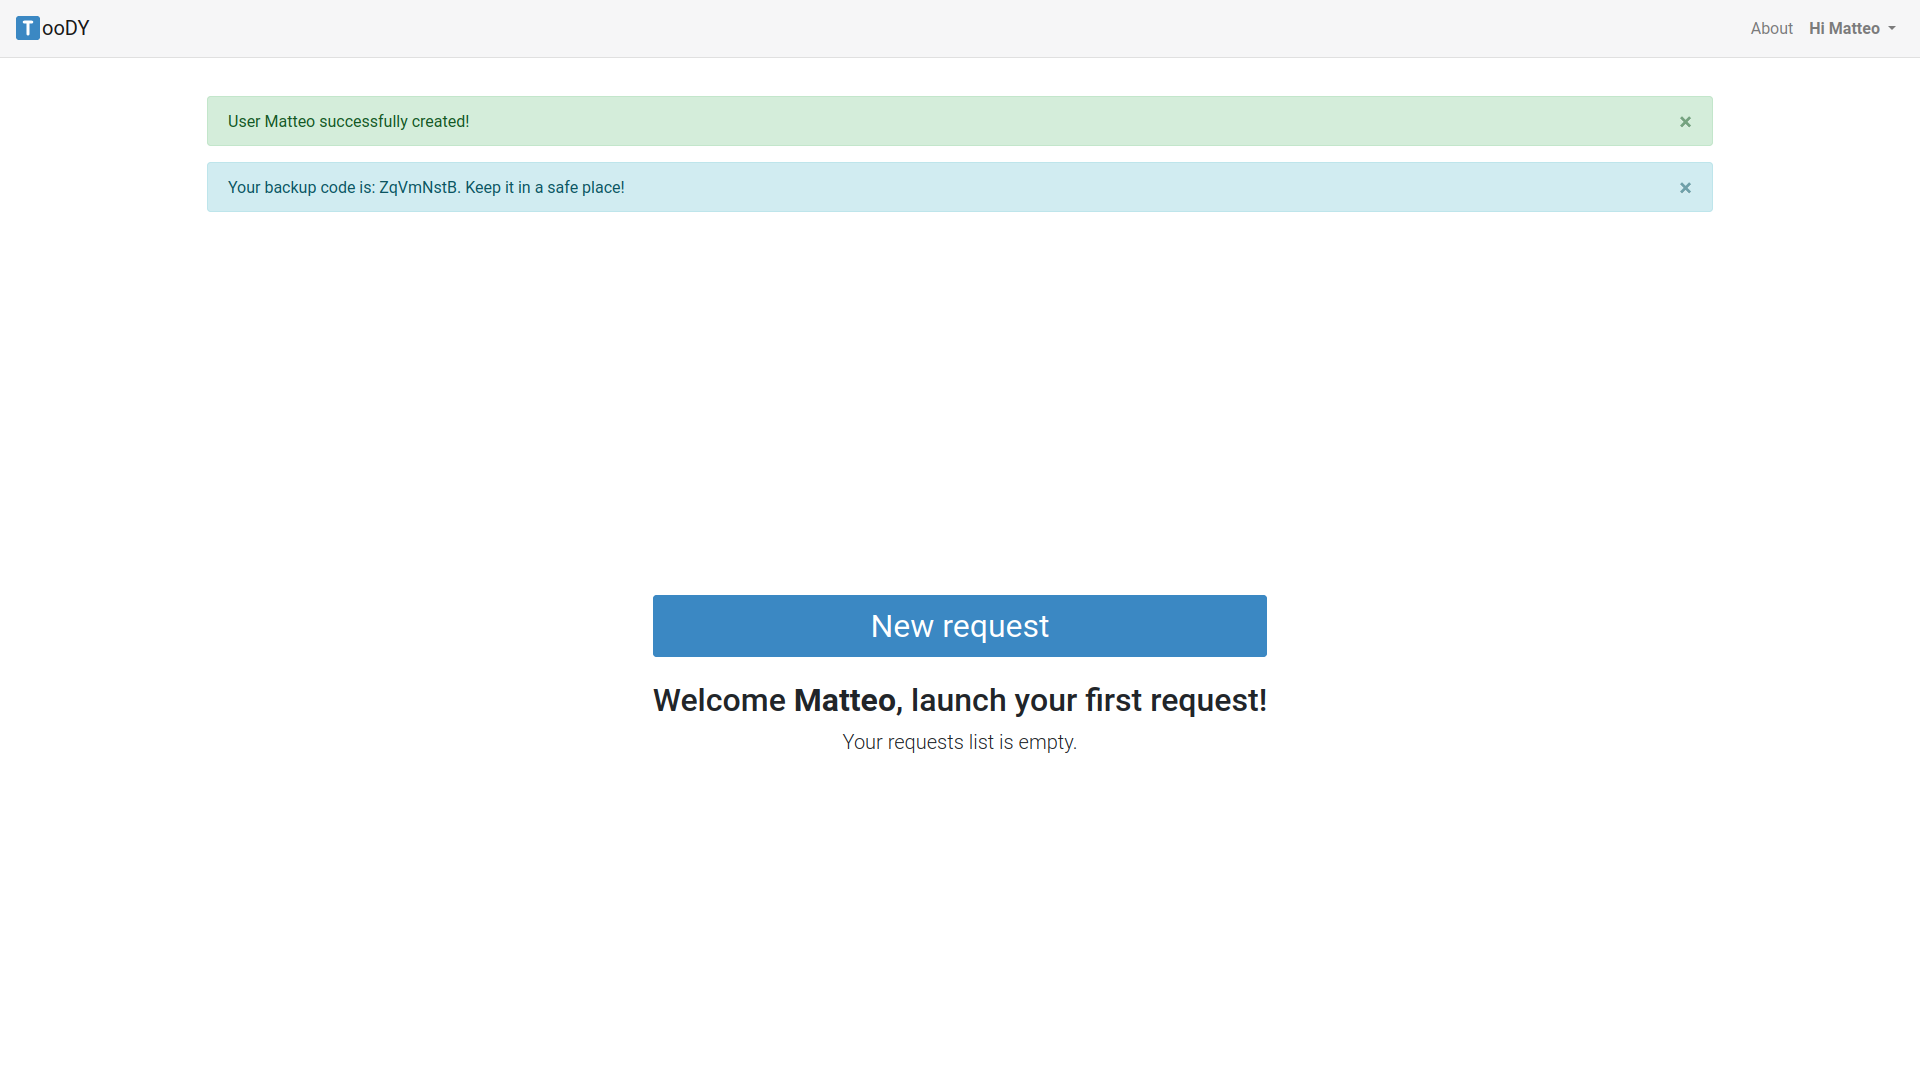
\includegraphics[width=1.0\textwidth]{pagina1-login.png}
\caption{\toody \textsf{main page}: login effettuato.}
\label{fig:pagina1-login}
\end{figure}

All'avvio dell'applicazione, l'utente si trova nella pagina di benvenuto che lo invita a registrarsi o effettuare il login. Non ci sono altre possibili interazioni, se non quella di visualizzare la pagina di \textit{about} con informazioni base sull'applicazione.

Nel caso l'utente si sia appena registrato, \toody lo informa\footnote{Le informazioni vengono recapitate all'utente tramite \textit{flash-texts}: strumento che \flask mette a disposizione per inviare messaggi temporanei, destinati ad essere visualizzati una sola volta, come una notifica o un alert che scompare dopo che l'utente ha proseguito con un'altra richiesta.} del successo dell'operazione e gli fornisce il \textit{backup-code}\footnote{Al momento della registrazione, \toody produce un codice randomico di 8 caratteri associato all'utente. Il \textit{backup-code} può essere generato nuovamente usando la funzione \textit{new backup-code} presente all'interno del menù a tendina sulla barra principale.} da inserire al posto della password in caso di smarrimento di quest'ultima.

\begin{figure}[H]
\centering
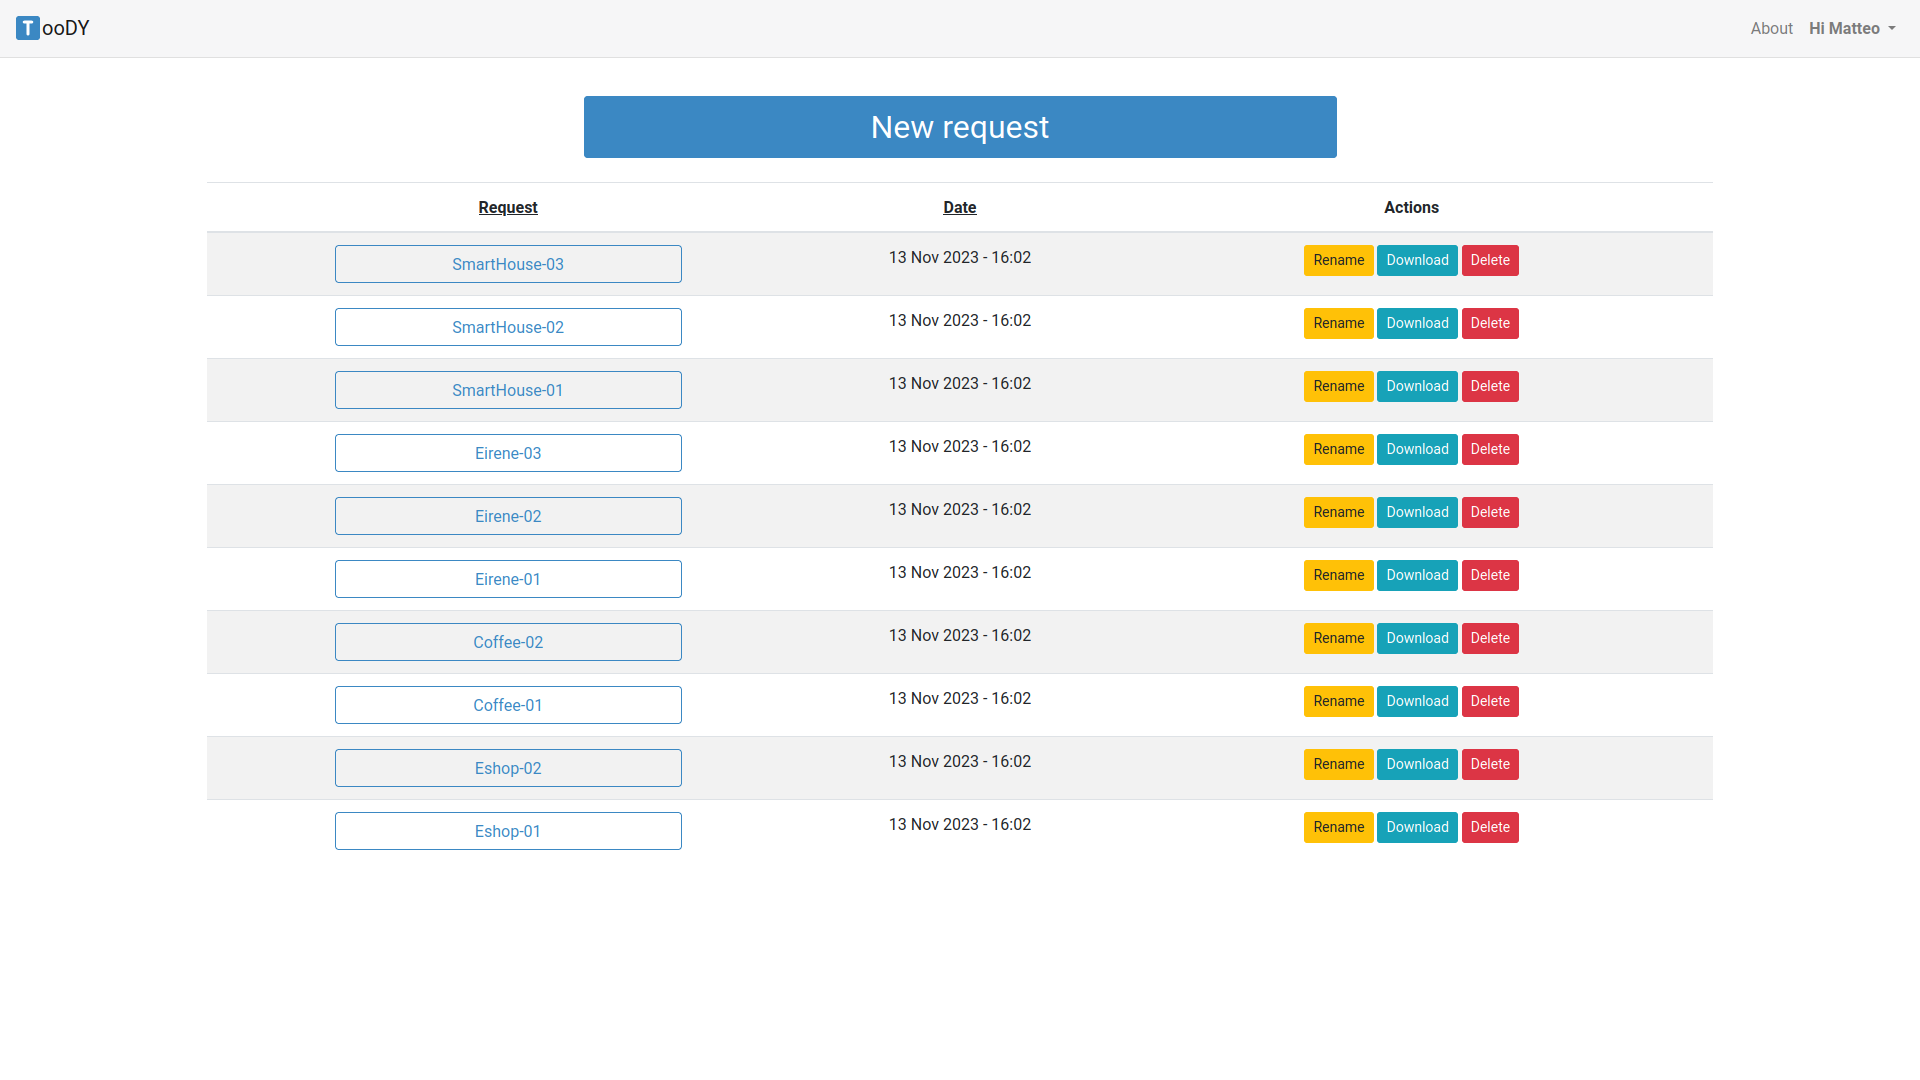
\includegraphics[width=1.0\textwidth]{pagina1-lista.png}
\caption{\toody \textsf{main page}: dashboard utente.}
\label{fig:pagina1-login}
\end{figure}

Effettuate le prime \textit{request}, la \textsf{main page} si trasforma in una dashboard personale. In questa pagina, l'utente può visualizzare l'elenco delle sue precedenti interazioni (ordinabili per nome o data), con la possibilità di rinominarle, scaricarle\footnote{La funzione di download permette di salvare sul proprio dispositivo un file \textit{zip} contenente il testo dei requisiti, il dizionario usato, i risultati dell'analisi e un file contenente il testo con i match evidenziati.} o eliminarle.

Le \textit{request} possono essere visualizzate cliccando sul singolo nome: questo reindirizza l'utente alla \textsf{second page} contenente tutti i dati dalla richiesta selezionata (testo, dizionario e risultati).


\newpage
\subsubsection{Gestione route principale}
\begin{lstlisting}[language=Python]
# La route principale può accettare
# un parametro `order` opzionale
@app.route("/")
@app.route("/<string:order>")
def main(order=None):
    # Controllo se l'utente corrente è autenticato
    # e ordino le richieste:
    #   `name_asc`  -> ordino per nome ascendente
    #   `name_desc' -> ordino per nome discendente
    #   `date_asc`  -> ordino per data ascendente
    #   `date_desc` -> ordino per data discendente
    if current_user.is_authenticated:
        if order == "name_asc":
            user_requests = (
                Request.query.filter_by(user_id=current_user.id)
                .order_by(Request.request_name.asc())
                .all()
            )
        elif order == "name_desc":
            user_requests = (
                Request.query.filter_by(user_id=current_user.id)
                .order_by(Request.request_name.desc())
                .all()
            )
        elif order == "date_asc":
            user_requests = (
                Request.query.filter_by(user_id=current_user.id)
                .order_by(Request.timestamp.asc())
                .all()
            )
        elif order == "date_desc":
            user_requests = (
                Request.query.filter_by(user_id=current_user.id)
                .order_by(Request.timestamp.desc())
                .all()
            )
        # Se non non specificato, recupera tutte le richieste
        # senza un ordine specifico
        else:
            user_requests = Request.query.filter_by(
                user_id=current_user.id
            ).all()

        # Renderizza il template `main.html` con le richieste
        # dell'utente e l'ordine specificato
        return render_template(
            "main.html", user_requests=user_requests, order=order
        )

    # Se l'utente non è autenticato,
    # renderizza il template `main.html`
    else:
        return render_template("main.html")
\end{lstlisting}


\subsection{\toody \textsf{second page}}
\label{sec:second-page}
La \textsf{second page} di \toody è il centro interattivo dell'applicazione, dove l'utente può caricare un documento, scegliere il dizionario e lanciare la richiesta di analisi del testo (\textit{Launch request}).

La prima parte della pagina è dedicata al caricamento dei dati e contiene due aree di testo: la più piccola è una semplice \texttt{textarea} ed è riservata al dizionario dei termini\footnote{\toody fornisce un elenco predefinito di voci da cercare, suddivise per categoria (\texttt{DISJ}, \texttt{OPTIONALITY}, \texttt{VAGUENESS} e \texttt{WEAKNESS}).}, mentre la più grande è un editor\footnote{L'editor in questione è \ace (\href{https://ace.c9.io/}{\textit{Ajax Cloud9 Editor}}): un code-editor versatile, realizzato per una efficiente integrazione con le applicazioni web. \ace offre un'esperienza non dissimile da quella propsta dai moderni desktop-editor e, nella configurazione scritta per \toody, permette di scegliere sia i keybindings \textsl{Default} che quelli \textsl{Vim-like}.} completo, destinato al testo dei requisiti.

\begin{figure}[H]
\centering
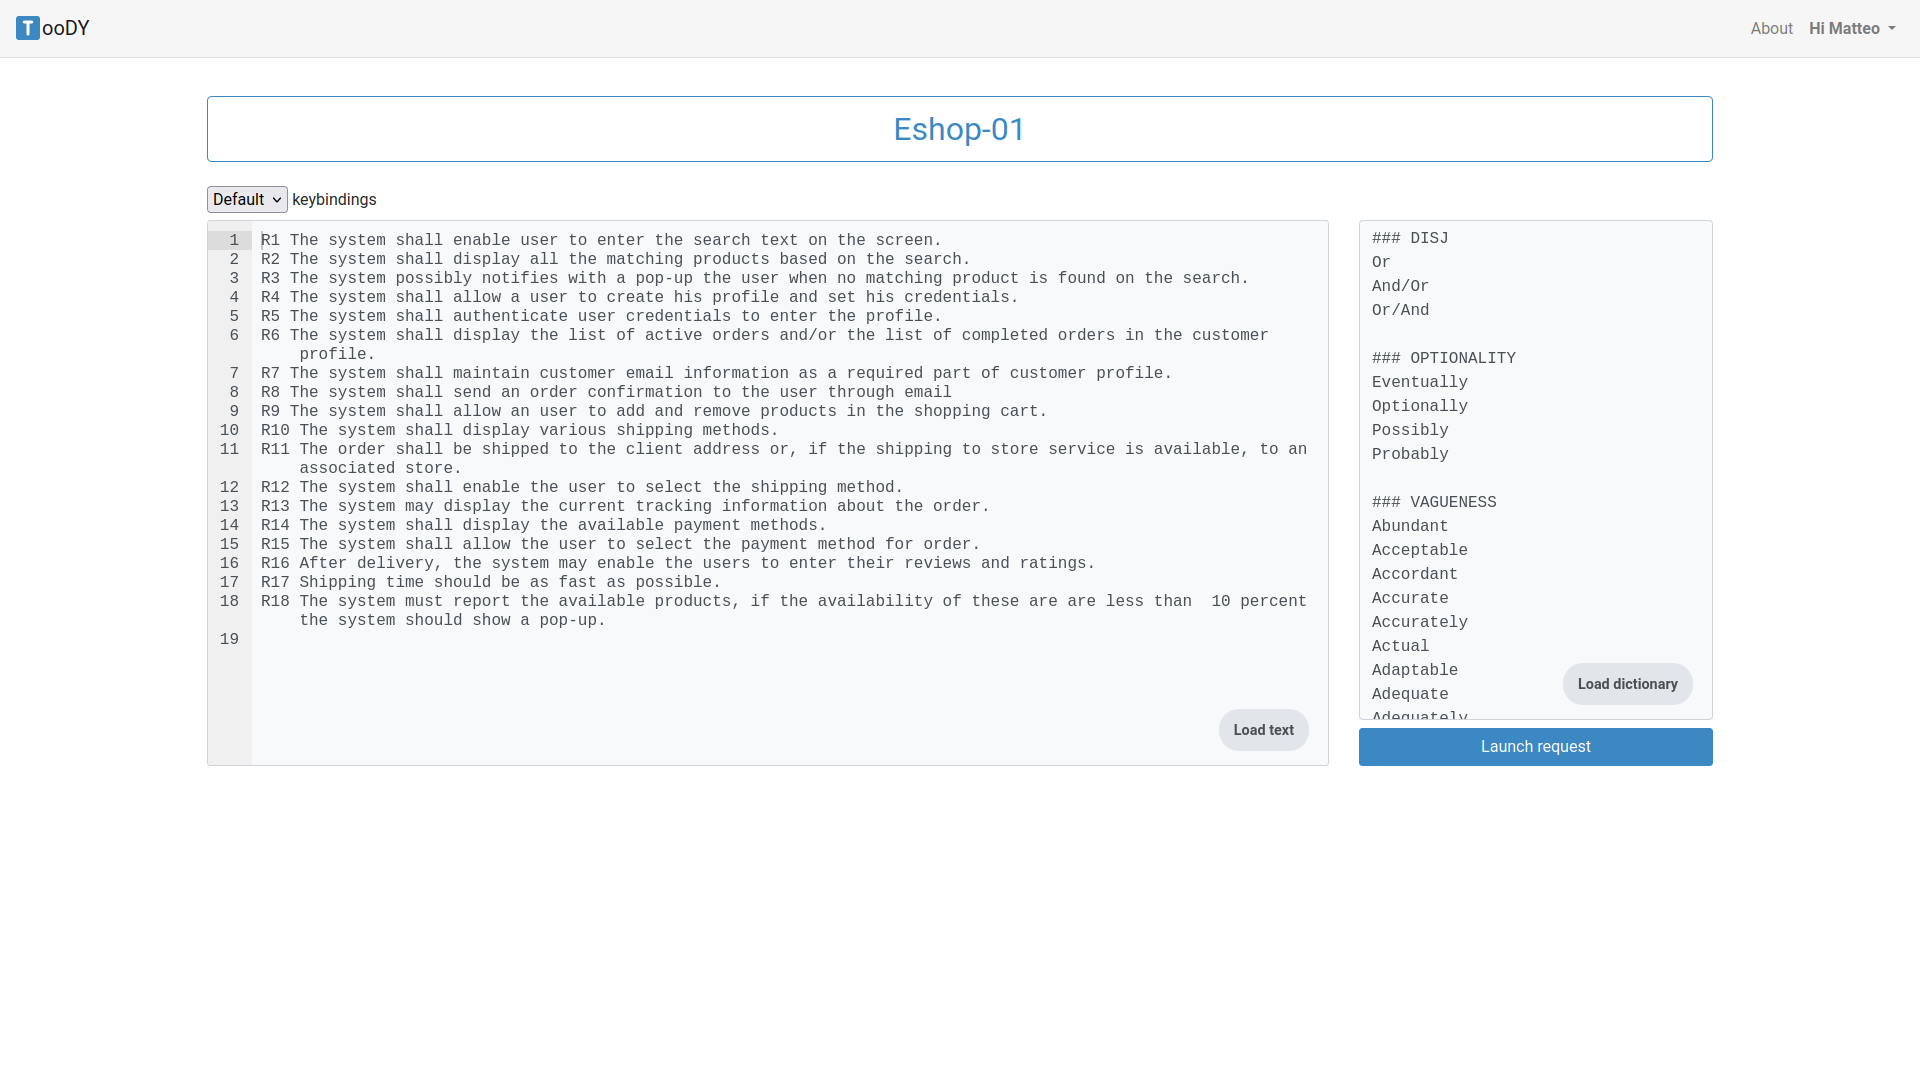
\includegraphics[width=1.0\textwidth]{pagina2-vuota.png}
\caption{\toody \textsf{second page}: nuova \textit{request}.}
\label{fig:pagina1-login}
\end{figure}

Nella seconda parte della pagina, sono mostrati i risultati dell'analisi. Dopo aver lanciato la \textit{request}, l'utente è immediatamente informato sui match lessicali, della forma passiva, delle congiunzioni verbali e delle frasi congiuntive\footnote{Questi quattro tipi di match corrispondono ai risultati trovati con le funzioni di analisi linguistica discusse in \cref{ch:parser}.}. I risultati così raggruppati sono organizzati in \textit{card} espandibili che forniscono contesto e numero di riga per ciascun match, offrendo una interfaccia utente facilmente navigabile.

\begin{figure}[H]
\centering
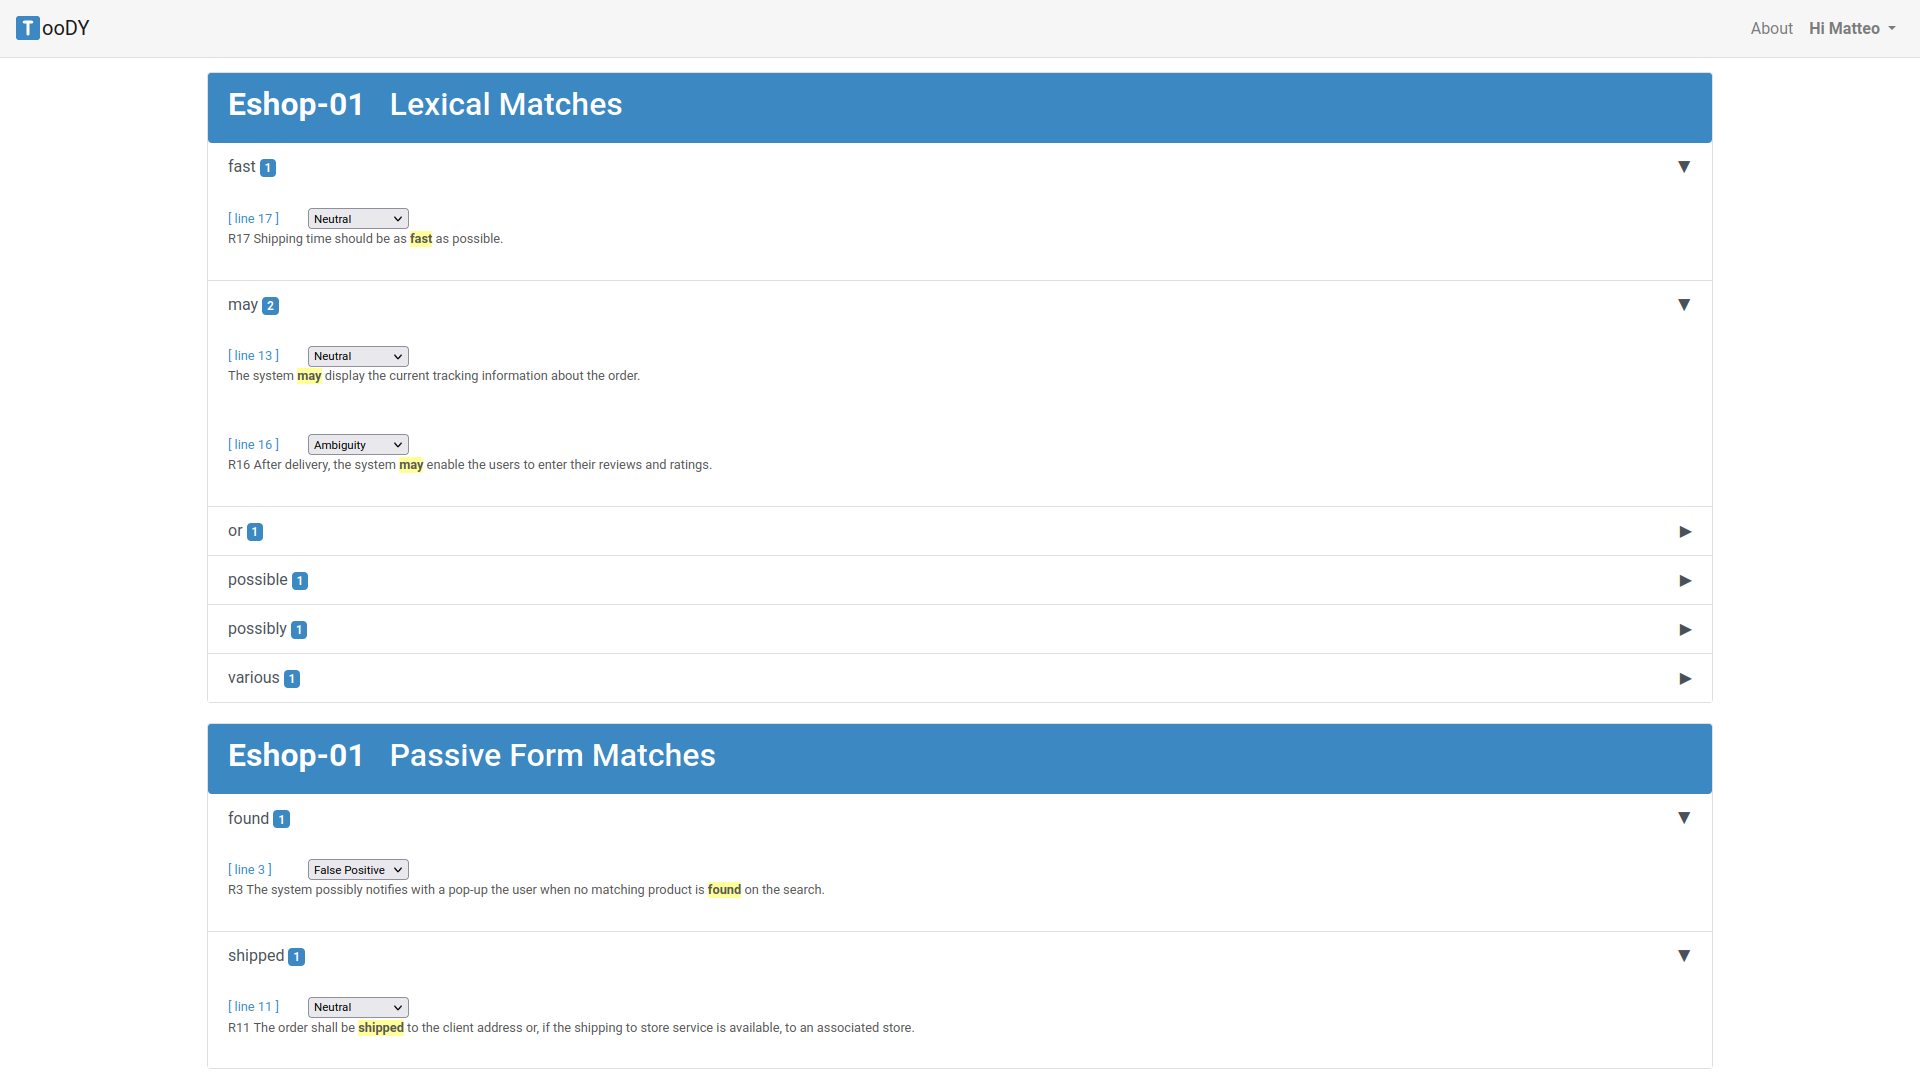
\includegraphics[width=1.0\textwidth]{pagina2-piena.png}
\caption{\toody \textsf{second page}: risultati \textit{request}.}
\label{fig:pagina1-login}
\end{figure}

Inoltre la pagina permette all'utente di interagire con i risultati e modificare le etichette adiacenti a ciascun match, scegliendo tra \textsf{Neutral}, \textsf{False Positive}, \textsf{Ambiguity} e \textsf{Variability}. Alla successiva \textit{request}, le etichette modificate saranno salvate nella variabile \texttt{memory}\footnote{\texttt{memory} rappresenta lo stato delle etichette di ciascun match. Questo consente all'utente di personalizzare le etichette e salvare le modifiche per le successive analisi, così che ogni richiesta salvata mantenga traccia del lavoro svolto.} e inviate al server assieme a testo e dizionario, così che gli algoritmi di analisi possano riconoscere ciascun nuovo match trovato e apporre subito l'eventuale etichetta corretta.


\subsubsection{Generazione dinamica delle \textit{card}}
\begin{lstlisting}[language=JavaScript]
function createResultCard(requestName, results, type) {
    // Inizio la creazione della card e imposto
    // la classe e lo stile per il margine superiore
    var resultDiv = document.createElement('div');
    resultDiv.className = "card";
    resultDiv.style.marginTop = "20px";

    // Definisco i nomi dei tipi di match e
    // assegno il nome del tipo del match basato sulla chiave
    var matchType = {
        "lexical": "Lexical Matches",
        "passive": "Passive Form Matches",
        "verbConjunction": "Verb Conjunction Matches",
        "conjunctionSentence": "Conjunction Sentence Matches"
    }[type] || "Unknown Type";

    // Definisco ID univoci per i contenuti collassabili
    const collapseId = `collapse${type}`;
    const headingId = `heading${type}`;

    // Creo intestazione card con trigger per collassare
    var headerDiv = document.createElement('div');
    headerDiv.className = "card-header collapsed-header";
    headerDiv.id = headingId;
    headerDiv.setAttribute("data-toggle", "collapse");
    headerDiv.setAttribute("data-target", `#${collapseId}`);
    headerDiv.setAttribute("aria-expanded", "true");
    headerDiv.setAttribute("aria-controls", collapseId);
    headerDiv.style.cursor = "pointer";
    headerDiv.innerHTML = `<h2><strong>${requestName}
                           </strong> &nbsp; ${matchType}</h2>`;
    resultDiv.appendChild(headerDiv);

    // Contenuto collassabile con i risultati
    var collapseDiv = document.createElement('div');
    collapseDiv.className = "collapse";
    collapseDiv.id = collapseId;
    collapseDiv.setAttribute("aria-labelledby", headingId);

    // Creo gruppo di elementi della lista
    // che conterrà i match individuali
    var listGroup = document.createElement('ul');
    listGroup.className = "list-group list-group-flush";

    // Funzione necessaria per la creazione di
    // un elemento della lista per ciascun match
    const createListItem = (key, resultsArray) => {
        // Creo un elemento della lista per
        // contenere i risultati del match
        const listItem = document.createElement('li');
        listItem.className = "list-group-item list-group-item-action";

        // ...
        // Costruisco la stringa HTML per il contesto del match
        let contextString = '';
        resultsArray.forEach(result => {
            // Genero codice HTML per le opzioni con
            // l'attributo `selected` appropriato
            let optionsHtml = `
                <option value="neutral" ...
                <option value="false_positive" ...
                <option value="ambiguity" ...
                <option value="variability" ...`;

            // Contesto in cui il match è stato trovato
            // già formattato in HTML
            contextString += `
                <div class="word-context">
                    ...
                </div>`;
        });

        // Inserisco il match e il badge nell'elemento della lista
        listItem.innerHTML = `<span>${key} <span class="badge ..."`

        // Aggiungo l'icona di espansione (>>)
        // per visualizzare il contesto
        const foldIcon = document.createElement('span');
        foldIcon.className = "fold-icon";
        foldIcon.setAttribute("data-toggle", "collapse");
        foldIcon.setAttribute("data-target", `#${contextId}`);
        foldIcon.setAttribute("aria-expanded", "false");
        foldIcon.setAttribute("aria-controls", contextId);
        foldIcon.innerHTML = '>>';
        foldIcon.addEventListener('click', function() {
            if (foldIcon.classList.contains('expanded')) {
                foldIcon.classList.remove('expanded');
            } else {
                foldIcon.classList.add('expanded');
            }
        });

        listItem.appendChild(foldIcon);

        // Aggiungo il contesto a quello originale
        const contextDiv = document.createElement('div');
        contextDiv.id = contextId;
        contextDiv.className = 'collapse';
        contextDiv.innerHTML = contextString;
        listItem.appendChild(contextDiv);

        // Restituisco l'elemento della lista
        return listItem;
    }

    // Per ogni risultato nell'insieme dei dati,
    // creo un elemento della lista per rappresentarlo
    for (let key in results) {
        listGroup.appendChild(createListItem(key, results[key]));
    }

    // Aggiungo il gruppo degli elementi della lista al
    // contenuto collassabile e quest'ultimo alla card
    collapseDiv.appendChild(listGroup);
    resultDiv.appendChild(collapseDiv);

    // Restituisco l'elemento creato
    return resultDiv;
}
\end{lstlisting}


\section{Funzionamento dell'applicazione}
% Per eseguire l'analisi del documento dei requisiti, l'utente interagisce con l'applicazione inserendo \torevise{il testo da analizzare e indicandi quale dizionario usare, altrimenti sembra vada copiaincollato anche il dizionario. Poi non chiarisci se anche per l'analisi sintattica l'utente dà delle indicazioni su quale fare o meno. E in caso, perché per i dizionari l'utente sceglie e per l'analisi sintattica no? va detto} testo e dizionario\footnote{La funzione \texttt{lexical\_analyser} (esaminata nella \cref{subsec:parser_lessicale}) esegue l'analisi lessicale del testo e richiede un dizionario dei termini da cercare. L'utente dispone di un dizionario default che può essere eventualmente modificato o sostituito.} nei campi preposti e lanciando la \textit{request}. Queste azioni vengono gestite dinamicamente lato client dalla funzione \texttt{contaParole}, che raccoglie i testi inseriti dall'utente e invia al server una richiesta \http \post, usando la \javascript \texttt{Fetch} \api\footnote{L'\api \texttt{Fetch} di \javascript è una moderna interfaccia di programmazione per effettuare richieste \http asincrone da un web-client a un server. In sostanza, consente di inviare e ricevere dati tra client e server in modo efficiente e flessibile.}.
All'apertura della \textsf{second page} (\cref{sec:second-page}), l'utente si trova a interagire con due aree di inserimento: una per il testo del documento dei requisiti e l'altra per il dizionario dei termini.

L'area preposta all'inserimento del testo è inizialmente vuota e l'utente può riempirla caricando un file \texttt{.txt} dal prorio dispositivo o scrivendo direttamente il contenuto. Un dizionario è già presente nell'area dedicata al momento dell'apertura (vedi \cref{app:dizionario}), \toody consente eventualmente di modificarlo o sostituirlo con uno nuovo.
% Il medesimo procedimento è valido anche per il dizionario, con la differenza che \toody ne fornisce uno predefinito già caricato nell'area dedicata (vedi \cref{app:dizionario}).
La scelta di usare un dizionario personalizzato per l'analisi lessicale, risiede nella volontà di consentire all'utente di guidare la ricerca in base alle proprie esigenze e al contesto del documento dei requisiti.

Una \textit{request} esegue sia l'analisi lessicale (\cref{subsec:parser_lessicale}), che quelle sintattiche (\cref{subsec:parser_forma_passiva,subsec:parser_congiunzioni_verbali,subsec:analizzatore_congiunzioni}).


\subsection{Invio della richiesta al server}
Lanciata la \textit{request}, le azioni vengono gestite dinamicamente lato client dalla funzione \texttt{contaParole}: essa raccoglie testo e dizionario inseriti dall'utente nelle aree preposte e invia al server una richiesta \http \post, usando la \javascript \texttt{Fetch} \api\footnote{L'\api \texttt{Fetch} di \javascript è una moderna interfaccia di programmazione per effettuare richieste \http asincrone da un web-client a un server. In sostanza, consente di inviare e ricevere dati tra client e server in modo efficiente e flessibile.}.

La richiesta inviata dal client contiene il testo del documento dei requisiti, il dizionario dei termini per l'analisi lessicale, il nome della richiesta e un oggetto che conserva le informazioni sullo stato corrente dell'applicazione\footnote{L'oggetto in questione (\texttt{memory}) è un dizionario. Esso agisce come memoria per le etichette con le quali l'utente ha marcato i risultati visualizzati sulla pagina \html dopo l'ultimo utilizzo.}. Il server riceve la richiesta e la elabora utilizzando le funzionalità di parsing e analisi del linguaggio naturale fornite da \spacy, come approfondito nel \cref{ch:nlp}.

Una volta ottenuta la risposta dal server, la funzione \texttt{contaParole} procede con l'elaborazione dei dati ricevuti. Il codice \javascript genera dinamicamente una rappresentazione \html dei risultati, creando \textit{card} dei match lessicali e sintattici per ciascuna delle categorie analizzate: risultati dell'analisi lessicale, di quella sintattica in forma passiva, delle congiunzioni verbali e delle frasi congiuntive.

In conclusione l'applicazione si basa su una semplice struttura client-server che sfrutta le funzionalità di \spacy per l'analisi del linguaggio naturale e \flask per la gestione delle richieste \http. Il server si concentra sull'elaborazione dei dati, mentre il client si occupa della presentazione dei risultati e dell'interazione con l'utente.


\subsubsection{Codice richiesta}
\begin{lstlisting}[language=JavaScript]
function contaParole() {
    // Raccolgo il testo dall'editor,
    // il dizionario e il nome della richiesta
    var content1 = editor.getValue();
    var content2 = document.getElementById("content2").value;
    var requestName = document.getElementById("requestName").value;

    // Controllo se tutti i campi sono stati compilati
    // ed eventualmente mostro un messaggio di errore
    if (!content1 || !content2 || !requestName) {
        $('#incompleteFieldsModal').modal('show');
        return;
    }

    // Invio una richiesta POST al server:
    // specifico metodo (POST), il tipo di contenuto (JSON)
    // e converto i dati della richiesta in formato JSON
    fetch('/conta-parole', {
        method: 'POST',
        headers: {
            'Content-Type': 'application/json',
        },
        // Aggiungo `memory` al corpo della richiesta
        body: JSON.stringify({
            'content1': content1,
            'content2': content2,
            'requestName': requestName,
            'memory': memory
        }),
    })
    .then(response => {
        console.log("Risposta dal server");
        return response.json();
    })
    .then(data => {
        console.log("Dati ricevuti");
        console.log(data);
        var resultsDiv = document.getElementById('results');
        resultsDiv.innerHTML = '';


        // Aggiungo un separatore
        var initialSeparator = document.createElement('div');
        initialSeparator.className = "resize-handler";
        resultsDiv.appendChild(initialSeparator);

        // Aggiungo i risultati lessicali
        // alla pagina se presenti
        if (data.lexical_results &&
            Object.keys(data.lexical_results.results).length) {
            console.log("CHECKMARK");
            let lexicalCard = createResultCard(
                requestName,
                data.lexical_results.results,
                "lexical"
            );
            resultsDiv.appendChild(lexicalCard);
        }

        // Aggiungo i risultati in forma passiva
        // alla pagina se presenti
        if (data.passive_form_results &&
            Object.keys(data.passive_form_results.results).length) {
            let passiveCard = createResultCard(
                requestName,
                data.passive_form_results.results,
                "passive"
            );
            resultsDiv.appendChild(passiveCard);
        }

        // Aggiungo i risultati delle congiunzioni verbali
        // alla pagina se presenti
        if (data.verb_conjunction_results &&
            Object.keys(data.verb_conjunction_results.results)
                  .length) {
            let verbConjunctionCard = createResultCard(
                requestName,
                data.verb_conjunction_results.results,
                "verbConjunction"
            );
            resultsDiv.appendChild(verbConjunctionCard);
        }

        // Aggiungo i risultati delle frasi congiuntive
        // alla pagina se presenti
        if (data.conjunction_sentence_results &&
            Object.keys(data.conjunction_sentence_results.results)
                  .length) {
            let conjunctionSentenceCard = createResultCard(
                requestName,
                data.conjunction_sentence_results.results,
                "conjunctionSentence"
            );
            resultsDiv.appendChild(conjunctionSentenceCard);
        }

        // Resetto il nome della richiesta
        // dopo la visualizzazione dei risultati
        document.getElementById("requestName").value = "";
    });
}
\end{lstlisting}


\subsection{Costruzione e invio della risposta al client}
Il server \toody è configurato per rispondere alle richieste \http \post alla \textit{route}\footnote{In \flask una \textit{route} è una funzione che viene associata a una \URL. In questo caso, la \textit{route} è associata all'\URL \texttt{/conta-parole} e accetta solo richieste \post.\\
Le \textit{route} vengono utilizzate per instradare le richieste \http alle funzioni appropriate. In questo caso, la funzione \texttt{conta\_parole} verrà chiamata quando viene ricevuta una richiesta \post all'\URL \texttt{/conta-parole} e potrà eseguire l'operazione desiderata.} \texttt{/conta-parole}. Quando il server riceve una richiesta da questo endpoint, la funzione \texttt{conta\_parole} viene invocata.

In questa fase, la richiesta viene prima decodificata e analizzata per assicurarsi che contenga dati validi in formato \json, poi la funzione estrae i vari elementi dalla richiesta, rispondendo con un errore in caso di dati mancanti o invalidi.

Usando la libreria \spacy, il testo dei requisiti viene trasformato in un doc-object, e vengono lanciate le funzioni di analisi linguistica\footnote{Le funzioni di analisi linguistica qui utilizzate sono quelle analizzate in \cref{ch:parser} e comprendono diversi aspetti dell'elaborazione del linguaggio naturale. Ciascuna di queste funzioni restituisce un dizionario contenente i match trovati e le informazioni necessarie per evidenziarli nel testo dei requisiti.}.

Al completamento delle funzioni, il server archivia i risultati delle analisi in un database insieme ad altri dettagli della richiesta: questo permette di conservare la cronologia delle richieste effettuate e recuperare i risultati in un secondo momento per revisioni o analisi future.

Infine, il server prepara una risposta in formato \json, contenente un dizionario che riporta i risultati delle analisi di ciascuna funzione, e la restituisce al client.


\subsubsection{Codice risposta}
\begin{lstlisting}[language=Python]
# Definisco la route `/conta-parole` che
# accetta solo richieste POST
@app.route("/conta-parole", methods=["POST"])
def conta_parole():
    # Estraggo i dati JSON dalla richiesta HTTP POST
    data = request.json

    # Verifico la presenza di dati nella richiesta e
    # restituisco un errore se i dati JSON non sono validi
    if not data:
        return jsonify({"error": "Invalid JSON data"}), 400

    # Estraggo i dati specifici dalla richiesta JSON:
    # testo dei requisiti, dizionario dei termini,
    # nome della richiesta e stato corrente dell'applicazione
    content1 = data.get("content1", "")
    content2 = data.get("content2", "")
    request_name = data.get("requestName", "")
    memory = data.get("memory", {})

    # Estraggo i sotto-dizionari specifici dall'oggetto `memory`
    lexical_memory = memory.get("lexical", {})
    passive_memory = memory.get("passive", {})
    verb_conj_mem = memory.get("verbConjunction", {})
    conj_sent_mem = memory.get("conjunctionSentence", {})

    # Creo un doc-object spaCy dal testo dei requisiti
    doc_requisiti = nlp(content1)

    # Chiamo le funzioni di analisi linguistica
    lexical_results = lexical_analyser(
        doc_requisiti, content1, content2, lexical_memory
    )
    passive_results = passive_form_parser(
        doc_requisiti, content1, passive_memory
    )
    verb_conj_results = verb_conjunction_parser(
        doc_requisiti, content1, verb_conj_mem
    )
    conj_sent_results = conjunction_sentence_analyser(
        doc_requisiti, content1, conj_sent_mem
    )

    # Se l'utente è autenticato, archivio i dati:
    # combino tutti i risultati delle analisi e
    # creo un nuovo record di richiesta nel database
    if current_user.is_authenticated:
        combined_results = {
            "lexical_results": lexical_results,
            "passive_form_results": passive_results,
            "verb_conjunction_results": verb_conj_results,
            "conjunction_sentence_results": conj_sent_results,
        }
        new_request = Request(
            content1=content1,
            content2=content2,
            user_id=current_user.id,
            request_name=request_name,
            lexical_total_matches=len(lexical_results),
            passive_total_matches=len(passive_results),
            verb_conjunction_total_matches=len(verb_conj_results),
            conjunction_sentence_total_matches=len(conj_sent_results),
            results=json.dumps(combined_results, indent=4),
            memory_data=json.dumps(memory),
        )
        db.session.add(new_request)
        db.session.commit()

    # Restituisco una risposta al client in
    # formato JSON, con i risultati delle analisi
    return jsonify(
        {
            "lexical_results": {
                "total_matches": len(lexical_results),
                "results": lexical_results,
            },
            "passive_form_results": {
                "total_matches": len(passive_results),
                "results": passive_results,
            },
            "verb_conjunction_results": {
                "total_matches": len(verb_conj_results),
                "results": verb_conj_results,
            },
            "conjunction_sentence_results": {
                "total_matches": len(conj_sent_results),
                "results": conj_sent_results,
            },
        }
    )
\end{lstlisting}


% \newpage
\subsubsection{Codice classe \texttt{Request}}
\begin{lstlisting}[language=Python]
class Request(db.Model):
    # Chiave primaria della tabella `Request` (univoca per richiesta)
    id = db.Column(db.Integer, primary_key=True)

    # Campi contenenti testo e dizionario inviati dall'utente
    content1 = db.Column(db.Text, nullable=False)
    content2 = db.Column(db.Text, nullable=False)

    # Campi per memorizzare il numero totale di corrispondenze
    lexical_total_matches = db.Column(db.Integer, nullable=True)
    passive_total_matches = db.Column(db.Integer, nullable=True)
    verb_conj_total_matches = db.Column(db.Integer, nullable=True)
    conj_sentence_total_matches = db.Column(db.Integer, nullable=True)

    # Qui sotto i campi per memorizzare i risultati delle analisi:
    #   results      -> JSON con i risultati delle analisi
    #   user_id      -> chiave che associa richiesta e utente
    #   request_name -> nome personalizzato richiesta
    #   timestamp    -> timestamp alla creazione della richiesta
    #   memory_data  -> dizionario che mantiene lo stato dell'analisi
    results = db.Column(
        db.Text, nullable=True
    )
    user_id = db.Column(
        db.Integer, db.ForeignKey("user.id"), nullable=False
    )
    request_name = db.Column(
        db.String(150), nullable=False, default="Unnamed Request"
    )
    timestamp = db.Column(
        db.DateTime, nullable=False, default=datetime.now(local_tz)
    )
    memory_data = db.Column(
        db.Text, nullable=True
    )
\end{lstlisting}


\section{Gestione degli utenti}
L'applicazione \toody è pensata per essere uno strumento di lavoro indipendente che permette all'utente di operare in autonomia senza la necessità di software ausiliari.

L'aspetto chiave per ottenere uno strumento del genere è quello di organizzare una gestione degli utenti che provveda non solo alle classiche funzionalità di accesso all'account (registrazione, login/logout, cancellazione, cambio password), ma anche alla possibilità di salvare e recuperare le \textit{request} effettuate.

L'archiviazione delle richieste permette agli utenti di mantenere un registro delle loro attività e recuperare analisi precedenti: un database conserverà quindi le informazioni relative a ciascuna richiesta, garantendo all'utente di visualizzare i risultati e scaricare i file relativi a una singola \textit{request}.


\subsubsection{Codice classe \texttt{User}}
\begin{lstlisting}[language=Python]
class User(UserMixin, db.Model):
    # ID univoco per ogni utente, usato
    # come chiave primaria nel database
    id = db.Column(db.Integer, primary_key=True)

    # Qua sotto i campi che memorizzano i dati utente:
    #   username        -> nome utente (unnico e non nullo)
    #   password        -> password utente (cifrata, non nulla)
    #   backup_code     -> codice di backup (randomico, opzionale)
    #   last_login_date -> data ultimo login (opzionale)
    #   last_activity   -> data ultima attività (opzionale)
    username = db.Column(db.String(150), unique=True, nullable=False)
    password = db.Column(db.String(150), nullable=False)
    backup_code = db.Column(db.String(150), nullable=True)
    last_login_date = db.Column(db.DateTime, nullable=True)
    last_activity = db.Column(db.DateTime, nullable=True)

    # Relazione con la tabella delle richieste (Request)
    # `backref` -> crea un attributo inverso nella classe Request
    #              chiamato `author`
    # `lazy`    -> definisce come i dati correlati vengono caricati
    # `cascade` -> gestisce la cancellazione dei dati correlati
    #              in modo automatico
    requests = db.relationship(
        "Request", backref="author", lazy=True,
        cascade="all, delete-orphan"
    )

    # Funzione per impostare la password dell'utente
    # (usa `generate_password_hash` per crittografare la password)
    def set_password(self, password):
        self.password = generate_password_hash(
            password, method="sha256"
        )

    # Funzione per verificare la correttezza della password
    # (usa `check_password_hash` per confrontare le password)
    def check_password(self, password):
        return check_password_hash(self.password, password)
\end{lstlisting}


\subsection{Registrazione utente}
La funzione \texttt{register} gestisce il processo di creazione di un nuovo account. Quando l'utente compila e invia il form di registrazione, la funzione verifica la correttezza della password inserita e la validità dello username scelto (eventualmente notificando l'utente).

Completata la registrazione, l'utente viene autenticato automaticamente e informato del successo dell'operazione. \toody invia il \textit{backup-code} da usare in fase di login al posto della password.

\subsubsection{Codice registrazione}
\begin{lstlisting}[language=Python]
# Definisco la route `/register` che
# accetta richieste GET e POST
@app.route("/register", methods=["GET", "POST"])
def register():
    # Se l'utente è già autenticato,
    # lo reindirizzo alla pagina principale
    if current_user.is_authenticated:
        return redirect(url_for("main"))

    # Se ricevuta una richiesta POST, significa che
    # il form di registrazione è stato inviato.
    if request.method == "POST":
        username = request.form["username"]
        password = request.form["password"]
        confirm_password = request.form["confirm_password"]

        # Controllo che password e conferma siano uguali;
        # controllo che lunghezza password rispetti il minimo
        if password != confirm_password:
            flash(
                "Passwords do not match. Please try again.",
                "warning"
            )
            return redirect(url_for("register"))
        if len(password) < MIN_PASSWORD_LENGTH:
            flash(
                f"Password must be at least {MIN_PASSWORD_LENGTH} "
                "characters long.", "danger"
            )
            return redirect(url_for("register"))

        existing_user = User.query.filter_by(
            username=username
        ).first()

        # Controllo che l'utente non esista già
        if existing_user:
            flash(
                f"User {username} already exists. "
                "Choose a different username.", "danger"
            )
            return redirect(url_for("register"))

        # Cifro la password, creo un nuovo utente
        # e lo inserisco nel database
        hashed_password = generate_password_hash(
            password, method="sha256"
        )
        backup_code = generate_random_string(8)
        new_user = User(
            username=username, password=hashed_password,
            backup_code=backup_code
        )
        db.session.add(new_user)
        db.session.commit()

        # Autentico il nuovo utente e lo reindirizzo
        # alla pagina principale
        login_user(new_user)
        flash(f"User {username} successfully created!", "success")
        flash(
            f"Your backup code is: {backup_code}. "
            "Keep it in a safe place!", "info"
        )
        return redirect(url_for("main"))

    # Se ricevuta una richiesta GET, renderizza
    # il template HTML per la registrazione
    return render_template("register.html")
\end{lstlisting}


\subsection{Login utente}
Il server \flask gestisce il processo di autenticazione attraverso la funzione \texttt{login}. Essa verifica le credenziali inserite nel form di login, dove l'utente potrà inserire la propria password o il \textit{backup-code} generato alla registrazione\footnote{Se un utente dovesse accedere a \toody usando il proprio \textit{backup-code}, a login effettuato, verrà generata randomicamente una nuova password e mostrata con un \textit{flash-text}. L'utente potrà cambiarla in un qualsiasi momento usando la funzione \textit{Change password} presente nel menù a tendina sulla barra principale.}. Un \textit{flash-text} informativo annuncerà il successo dell'operazione e l'utente verrà reindirizzato alla \textsf{main page}.


\subsubsection{Codice login}
\begin{lstlisting}[language=Python]
# Definisco la route `/login` che
# accetta richieste GET e POST
@app.route("/login", methods=["GET", "POST"])
def login():
    # Se l'utente è già autenticato, lo
    # reindirizzo alla pagina principale
    if current_user.is_authenticated:
        return redirect(url_for("main"))

    # Gestisco la richiesta di login quando
    # l'utente invia il form
    if request.method == "POST":

        # Usando lo username inserito, cerco
        # l'utente nel database
        user = User.query.filter_by(
            username=request.form["username"]
        ).first()

        # Controllo che l'utente esista
        # e che stia usando il backup-code
        if user and user.backup_code == request.form["password"]:
            new_password = generate_random_string(8)
            user.set_password(new_password)
            user.last_login_date = datetime.utcnow()
            user.last_activity = datetime.utcnow()
            db.session.commit()

            # Effettuo il login dell'utente
            # e mostro un flash-text
            login_user(user)
            flash(
                f"Hi {user.username}, you've logged in with "
                "the backup code!", "warning"
            )
            flash(
                f"Your new password is {new_password}. "
                "Please change it as soon as possible!", "info"
            )
            return redirect(url_for("main"))

        # Se l'utente esiste e sta usando la password,
        # effettuo il login e mostro un flash-text
        elif user and user.check_password(request.form["password"]):
            login_user(user)
            user.last_login_date = datetime.utcnow()
            user.last_activity = datetime.utcnow()
            db.session.commit()
            flash(
                f"Hi {user.username}, you've successfully logged in",
                "success"
            )
            return redirect(url_for("main"))

        # Se l'accesso fallisce,
        # mostro un flash-text di errore
        else:
            flash(
                "Login failed. Please check username and password.",
                "danger"
            )

    # Se il metodo è GET o il login non è andato a buon fine,
    # reinidirizzo l'utente alla pagina di login
    return render_template("login.html")
\end{lstlisting}


\subsection{Logout utente}
Affinchè l'applicazione possa disconnettere gli utenti loggati, il server dispone della funzione \texttt{logout}: una procedura che usa il meccanismo \textsf{Flask-Login}\footnote{Quando un utente effettua il login, \textsf{Flask-Login} memorizza un identificatore univoco (\textsf{ID}) per l'utente nella sessione del browser, che sarà poi accessibile nelle richieste \http successive. Questa informazione è salvata in un cookie sicuro che il browser invia automaticamente al server insieme ad ogni richiesta.\\
Nel momento in cui viene invocata \texttt{logout\_user}, \textsf{Flask-Login} cerca l'identificatore nella sessione attuale per determinare quale utente debba essere scollegato. Rimuove quindi l'\textsf{ID} dell'utente dalla sessione (pulendo ogni dato associato) e fa in modo che le richieste future non siano più autenticate come quell'utente.\\
Le sessioni in Flask sono protette e non possono essere facilmente manomesse dal client: questo garantisce che l'\textsf{ID} dell'utente nella sessione sia affidabile.}, messo a disposizione dal framework, per terminare la sessione dell'utente corrente. Dopo aver effettuato la disconnessione, \texttt{logout} non fa altro che mostrare un \textit{flash-text} di notifica e reindirizzare l'utente alla pagina principale.

La disconnesione dell'utente dalla sessione può avvenire anche in modo automatico: la funzione \texttt{heartbeat} si occupa di controllare periodicamente l'attività dell'utente e, se questo rimanesse inattivo per più di 30 minuti, la sessione verrebbe terminata automaticamente, l'utente informato con un \textit{flash-text} e reindirizzato alla pagina di login.


\subsubsection{Codice logout}
\begin{lstlisting}[language=Python]
# Definisco la route `/logout` che
# richiede l'autenticazione dell'utente
@app.route("/logout")
@login_required
def logout():
    # Salvo il nome dell'utente corrente
    # Lancio la funzione `logout_user()` di `flask-login`
    username = current_user.username
    logout_user()

    # Mostro un flash-text di notifica
    # e reindirizzo l'utente alla pagina principale
    flash(f"User {username} disconnected.", "info")
    return redirect(url_for("main"))
\end{lstlisting}


\subsubsection{Codice auto-logout}
\begin{lstlisting}[language=Python]
# Definisco la route `/heartbeat` che
# richiede l'autenticazione dell'utente
@app.route("/heartbeat")
@login_required
def heartbeat():
    # Ottengo l'orario corrente in UTC
    now = datetime.utcnow()

    # Se l'utente non ha effettuato alcuna richiesta negli
    # ultimi 30 minuti, lo disconnetto, mostro un flash-text
    # di notifica e reindirizzo l'utente alla pagina di login
    if (now - current_user.last_activity) > timedelta(minutes=30):
        logout_user()
        flash(
            "You have been logged out due to inactivity.", "warning"
        )
        return redirect(url_for("login"))

    # Se l'utente è attivo, restituisco una risposta vuota
    # con status-code 204 (No Content)
    return "", 204
\end{lstlisting}


\begin{mdframed}
\small
Nel client, integrato in \html tramite \jinja, è presente un frammento \javascript che chiama la route \texttt{/heartbeat} a intervalli regolari. Questa chiamata funge da meccanismo keep-alive per gli utenti attivi e da trigger per il logout automatico scatenato da \texttt{heartbeat} per quelli zombie.

\begin{lstlisting}[language=JavaScript]
// Se l'utente è autenticato, chiamo la route '/heartbeat'
// del server e imposto un intervallo di chiamata di 1 min.
if ({{ current_user.is_authenticated|tojson }}) {
    setInterval(function() {
        window.location.href = '/heartbeat';
    }, 1 * 60 * 1000);
}
\end{lstlisting}
\end{mdframed}


\subsection{Cancellazione utente}
Per una gestione completa degli utenti registrati su \toody, il server contiene funzioni per la rimozione degli account.

\texttt{unregister} esegue una semplice cancellazione di un account dall'applicazione. Dopo averne verificato l'identità, la funzione elimina l'account, disconnette l'utente, lancia un \textit{flash-text} di notifica ed esegue il reindirizzamento alla pagina principale.

\texttt{remove\_inactive\_users} è programmata per eliminare automaticamente gli account degli utenti inattivi da più di 15 giorni. Questa funzione è essenziale per mantenere il database pulito, rimuovendo account non più utilizzati.

\texttt{start\_scheduler} è responsabile dell'avvio di uno scheduler\footnote{La funzione \texttt{start\_scheduler} usa \texttt{BackgroundScheduler} per la gestione degli utenti inattivi. \texttt{BackgroundScheduler} è parte del modulo \href{https://apscheduler.readthedocs.io/en/stable/}{\textsf{APScheduler}} e consente di programmare l'esecuzione di compiti in determinati momenti o dopo intervalli di tempo specifici (con un funzionamento analogo ai cron-jobs Linux).\\
Nello specifico, questo scheduler esegue tutti i sui thread in background (senza interferire con il processo principale, né interrompere il normale flusso di esecuzione dell'applicazione) ed è persistente rispetto ai lavori pianificati (i processi schedulati vengono salvati nel database e ripristinati in caso di riavvio dell'applicazione).} in background che esegue periodicamente la funzione \texttt{remove\_inactive\_users}. Questo garantisce che la pulizia periodica degli utenti inattivi avvenga automaticamente.


% \newpage
\subsubsection{Codice cancellazione}
\begin{lstlisting}[language=Python]
# Definisco la route `/unregister` che
# accetta richieste POST e richiede
# l'autenticazione dell'utente
@app.route("/unregister", methods=["POST"])
@login_required
def unregister():
    # Recupero la password fornita dall'utente con il form e
    # trovo l'utente corrente nel database utilizzando il suo ID
    password = request.form["password"]
    user = User.query.filter_by(id=current_user.id).first()

    # Verifico che la password fornita sia corretta con
    # `check_password_hash` per confrontare la password cifrata
    if not check_password_hash(user.password, password):
        flash("Incorrect password. Please try again.", "danger")
        return redirect(url_for("main"))

    # Salvo il nome dell'utente, elimino l'utente
    # dal database e committo i cambiamenti
    username = current_user.username
    db.session.delete(current_user)
    db.session.commit()

    # Disconnetto l'utente utilizzando con `logout_user`,
    # mostro un flash-text di conferma e reindirizzo l'utente
    # alla pagina principale
    logout_user()
    flash(f"User {username} has been deleted.", "info")
    return redirect(url_for("main"))
\end{lstlisting}


\subsubsection{Codice auto-cancellazione}
\begin{lstlisting}[language=Python]
def remove_inactive_users():
    # Stabilisco una soglia calcolata come
    # il timestamp attuale meno 15 giorni
    threshold_date = datetime.utcnow() - timedelta(days=15)

    # Recupero tutti gli utenti che non hanno effettuato
    # l'accesso da prima della data soglia
    inactive_users = User.query.filter(
        User.last_login_date <= threshold_date
    ).all()

    # Scorro la lista degli utenti inattivi
    # e li elimina dal database
    for user in inactive_users:
        db.session.delete(user)
    db.session.commit()


def start_scheduler():
    # Nuovo scheduler in background
    scheduler = BackgroundScheduler()

    # Aggiungo un lavoro allo scheduler: la funzione
    # `remove_inactive_users` che verrà eseguita giornalmente
    # ed eliminerà gli utenti inattivi da più di 15 giorni
    scheduler.add_job(
        remove_inactive_users,
        "interval",
        days=1
    )

    # Avvio lo scheduler
    scheduler.start()
\end{lstlisting}


\newpage
\begin{mdframed}
\small
Il frammento di codice finale del server \flask è il punto di ingresso dell'applicazione. Qui, prima di lanciare l'applicazione, viene avviata la funzione \texttt{start\_scheduler}, assicurando che il meccanismo di pulizia degli account inattivi sia in funzione.

\begin{lstlisting}[language=Python]
if __name__ == "__main__":
    # Creo tutte le tabelle nel database e
    # avvio lo scheduler `BackgroundScheduler`
    with app.app_context():
        db.create_all()
        start_scheduler()

    # Avvio l'applicazione Flask
    app.run(debug=True)
\end{lstlisting}
\end{mdframed}


% PAGINA BIANCA
% \clearpage\thispagestyle{empty}
% \null\newpage


% CAPITOLO 6
\chapter{Conclusioni}
\label{ch:conclusioni}
In questo capitolo finale, ci proponiamo di riflettere sugli obiettivi inizialmente delineati per questo lavoro di tesi e valutare eventuali sviluppi futuri dell'applicazione ottenuta.

\subsubsection{Funzionamento \spl \& variabilità nei requisiti}
In questo elaborato è stata condotta un'analisi delle \textit{Software Product Lines}, con un focus particolare sul ruolo della variabilità nei documenti dei requisiti ed è stato possibile comprendere le dinamiche associate alla gestione della variabilità in questi contesti.

Sono stati evidenziati i principali indicatori di variabilità e l'impatto che questi comportano nel diagramma delle \textit{features} del sistema software.

\subsubsection{Tecniche di NLP \& funzionalità \spacy}
Ai fini di automatizzare la ricerca degli indicatori di variabilità nei requisiti, è stato necessario studiare le tecniche di \textit{Natural Language Processing} e utilizzare la libreria \spacy per eseguire analisi lessicale e sintattica.

La costruzione di un parser lessicale ha permesso la rilevazione di varibilità causata da indicatori di vaghezza, debolezza e opzionalità. Mentre l'implementazione di tre diversi analizzatori sintattici ha consentito di identificare la variabilità dovuta a forme passive, molteplicità e costrutti tipo \textit{if}, \textit{when}, \textit{where}.

Il prototipo di base, precedentemente sviluppato \cite{livi}, ha fornito un buon punto di partenza per la costruzione delle funzioni di analisi e, grazie a un lavoro di refactoring non banale, è stato possibile adattare il codice alle nuove funzionalità, pur mantenendo una buona efficienza.

\subsubsection{Costruzione web-app con \flask}
In ultimo, vista la necessità di fornire una interfaccia grafica allo strumento creato, una parte importante del lavoro ha riguardato la realizzazione di una interfaccia web, con l'impiego del framework \flask.

Questo ha permesso di trasformare un semplice prototipo iniziale da riga di comando, in un'applicazione web funzionale, migliorandone l'esperienza utente e rendendo \toody una piattaforma di lavoro completa, più accessibile agli utenti finali.

{\centering \rule{0.5\linewidth}{0.1pt} \par\vspace{0.25cm}}

Questo progetto di tesi ha affrontato con successo gli obiettivi prefissati, costruendo uno strumento di lavoro che permette di automatizzare la ricerca di variabilità nei requisiti e dimostrando come le tecniche di \nlp possano essere applicate nella modellazione delle linee dei prodotti software.

% \vspace{0.5cm}
Per quanto riguarda possibili \textsf{sviluppi futuri}, \toody potrebbe essere esteso aggiungendo la possibilità di scegliere la lingua con la quale effettuare le analisi e, vista la recente diffusione di \textit{Large Language Models}, sarebbe interessante affiancare alle funzioni sviluppate con \spacy un \textsl{LLM} che integri l'analisi dei costrutti sintattici per un risultato più completo. Con le nuove ricerche effettuate nel campo dei \textit{Large Language Models}, un loro impiego offrirebbe inoltre la possibilità di eseguire analisi semantica, consentendo il riconoscimento diretto dei punti di variabilità.


\begin{mdframed}
\small
Il codice sorgente dell'applicazione \toody è disponibile pubblicamente su GitHub all'indirizzo \url{https://github.com/matteogiorgi/toody}.
\end{mdframed}


% PAGINA BIANCA
% \clearpage\thispagestyle{empty}
% \null\newpage


\nocite{*}
\printbibliography


% PAGINA BIANCA
% \clearpage\thispagestyle{empty}
% \null\newpage


\appendix
\chapter{Dizionario}
\label{app:dizionario}
Il presente dizionario, qui allegato in appendice, è usato da \toody per l'analisi lessicale effettuata da \texttt{lexical\_parser}. Esso è una raccolta di termini suddivisi in categorie usati per la ricerca di indicatori di variabilità nei requisiti.

Può essere liberamente esteso aggiungendo voci alle categorie esistenti o creandone di nuove: ogni riga non vuota o che non inizi con il carattere \texttt{\#} è considerata una voce del dizionario.

Di seguito sono riportate le categorie del dizionario default di \toody, con i termini che le compongono\footnote{I termini sono qui elencati sottoforma di lista di stringhe separate da carattere bianco anzichè da newline, per motivi di spazio.}: vaghezza, debolezza, opzionalità e disgiunzione.


\subsubsection{Vagueness}
\begin{lstlisting}
Abundant Acceptable Accordant Accurate Accurately Actual Adaptable
Adequate Adequately Adjacent Advantageous Affordable Agile Agreeable
Ambitious Ambivalent Ample And So On Annoying Apparent Apposite
Appreciable Appropriate Appropriately Approximate Approximately
Apropos Apt Arduous Abstruse Abstrusely As Required Bad Badly
Baffled Beautiful Befitting Boring Bothersome Brief Briefly Broad
Broadly Businesslike Capable Capacious Careful Catchy Certain
Challenging Cheap Clean Clear Clearly Closely Coarse-Grained Coarse
Grained Coherent Colossal Comfortable Comfy Competent Complex
Complicated Concise Concisely Concordant Confident Conformable
Confused Congenial Congruent Congruous Considerable Consonant
Conspicuous Cost-Effective Cost Effective Cost-Efficient Cost
Efficient Counterfeit Counterintuitive Crucial Cryptic Cushy Decent
Deep Deeply Deficient Delicate Delicately Demanding Dependable
Desirable Detailed Detective Difficult Dirty Disagreeable Discordant
Disfigured Dishy Disordered Disorganised Disorganized Displeasing
Distant Doubtful Easily Easy Easygoing Economic Effective Effectively
Effectual Efficacious Efficient Efficiently Effortful Effortless
Elaborated Elegant Elementary Eligible Enough Etc.  Evident Expedient
Expeditious Expensive Explicable Extended Extensive Extraordinary
Fair Fair To Middling Fancy Fashionable Fast Fine Fine-Grained Fine
Grained Finely Fit Flexible Fluent Frail Fresh Fruitful Full-Size
Full Size Fundamental Futile Fuzzy Galling General Gentle Genuine
Giant Good Goodish Gross Hands-Down Hands Down Hard Hard-Fought Hard
Fought Hard-Hitting Hard Hitting Hardly Harmonious Harsh Heavy
Helpful Hostile Illegible Immediate Imminent Impartial Imperfect
Impertinent Impolite Important Impractical Impressive Improper Impure
Inaccurate Inaccurately Inadequate Inadequately Inappropriate
Inappropriately Incapable Incoherent Incompetent Incomprehensible
Incongruous Inconsiderable Inconsiderably Inconsiderately
Inconspicuous Indisputable Indisputably Ineffective Ineffectively
Ineffectual Inefficacious Inefficient Ineligible Inexpedient
Inexpensive Inexplicable Insecure Insecurely Insignificant
Insufficient Intense Interesting Intimately Intuitive Irrational
Irrelevant Irritating Just About Large Legible Light Limpid Logical
Long Loud Major Malapropos Manifest Massive Meager Meaningful
Meaningless Mediocre Middling Mild Minor Moderate Naive Narrow Nasty
Near Nearly Neat Nerve-Racking Nerve Racking Nerve-Wracking Nerve
Wracking Nettlesome Nice Nifty Nonspecific Noteworthy Obvious Of
Import Of Value Ordinary Organized Obscure Outsize Outsized Overlarge
Oversize Oversized Painless Passable Pat Perfect Pertinent Pesky
Plaguy Plain Pleasant Pleasing Pleasureful Polite Poor Possible
Practical Precarious Precise Pretty Problematic Prolix Prominent
Promptly Proper Properly Pure Qualified Quick Rapid Rational Raw
Reasonable Recent Recondite Relevant Reliable Remarkable Repulsive
Respectable Rich Risky Robust Rough Rough-And-Ready Rough And Ready
Roughly Sane Sapless Satisfactory Scanty Scarce Seamless Serious
Seriously Several Sharp Short Short-Handed Short Handed Shortly
Short-Staffed Short Staffed Sightly Significant Silly Simple
Simplified Simplistic Simply Slim Slow Slowly Slow-Moving Slow Moving
Small-Scale Small Scale Smart Smashing Smooth Smooth Smutty Solid
Some Sophisticated Sound Spacious Sparse Specific Speculative Speedy
Spontaneous Strange Stressful Strong Substantial Sufficient Suitable
Suited Superb Superficial Swell Synthetic Teasing Tedious Thick Thin
Tight Timesaving Tiny To The Point Today's Trenchant Trenchantly
Tricky Trivial Troublesome Unadaptable Unbefitting Unclear
Uncollectible Uncomfortable Uncomplicated Undemanding Undependable
Undermanned Underspent Understaffed Uneasy Uneffective Uneffectively
Unfair Unfit Unfruitful Unhelpful Unimportant Uninteresting
Unmistakable Unnatural Unpleasant Unqualified Unreliable
Unsatisfactory Unserviceable Unsound Unstable Unsubtle Unsuitable
Unsure Unsweet Unusable Unuseable Usable Useable Useful Useless
User-Friendly User Friendly Utile Utilizable Valuable Various Vast
Versatile Vexatious Vexing Virtually Voluminous Wasteful Weakly Well
Behaved Well Known Well-Known Well-Behaved Well Behaved Well-Founded
Well Founded Wide Widely Worthy
\end{lstlisting}


\subsubsection{Weakness}
\begin{lstlisting}
Can Could May Might Would
\end{lstlisting}


\subsubsection{Optionality}
\begin{lstlisting}
Eventually Optionally Possibly Probably
\end{lstlisting}


\subsubsection{Disjunction}
\begin{lstlisting}
Or And/Or Or/And
\end{lstlisting}


\end{document}
